\chapter{When do the effects of interaction happen? Interacting and disturbed galaxies in the COSMOS field}\label{chapter3}
\section{Abstract}
   Galaxy interaction and merging have fundamental impacts on galactic evolution. From increases in star formation, to morphology, to activation of nuclear activity, galaxy interaction is thought to play a role. However, at what point in the interaction do these effects occur? In this work, we break down a large sample of identified interacting galaxies and split them into four distinct stages based on their interaction morphology. Each stage captures a different part of the dynamical timescale of interaction; from the systems approaching each other to actually merging. We cross match this large sample with the COSMOS field to provide ancillary data and each galaxys' underlying parameters. We then investigate the relation between stage, mass, star formation, and nuclear activation. Using Kolmogorov-Smirnov tests, we find that the distribution of star formation rates rapidly changes with stage for an equivalent mass distribution. We find a rapidly shrinking red sequence with stage, and a large increase in the fraction of starburst galaxies at the point of coalescence. We also find that the fraction of active galactic nuclei is static through most of the interaction, until it dramatically increases at coalescence. We discuss these results, and compare them with the more prevalent stage diagnostic of projected separation between galaxy pairs. We find interesting behaviour that is morphology and stage dependent in our samples star formation rates which is not captured by only using the projected separation. We show that morphological stage and, more specifically, the point in time of the underlying dynamical timescale an interaction occupies is as important to consider as its projected separation. We conclude this work with discussions on how this could be applied to larger, more complete datasets of interacting galaxies with available ancillary data.

%%%%%%%%%%%%%%%%%%%%%%%%%%%%%%%%%%%%%%%%%%%%%%%%%%

%%%%%%%%%%%%%%%%% BODY OF PAPER %%%%%%%%%%%%%%%%%%

\section{Introduction}\label{introduction}
\noindent Galaxy interaction and merging is of fundamental importance to our current theories of galaxy formation and evolution. Our current cosmological theory, $\Lambda$CDM dictates that structure is expected to form and assemble hierarchically \citep{1978MNRAS.183..341W, 2001MNRAS.328..726S, 2013MNRAS.436.1765M}. Thus, understanding the underlying processes that occur in galaxy interaction and merging are paramount to understanding cosmological theories. It is well known that many underlying processes are triggered or enhanced due to galaxy interaction. The clearest result of interaction is the disruption of galactic morphology, the acceleration of disks to spheroidal systems and the formation of tidal features \citep{1972ApJ...178..623T, 1977ApJ...212..616T, 2005MNRAS.357..753G, 2009MNRAS.397..802H}, increases in star formation rates when compared to the general galaxy population \citep{1991ApJ...370L..65B, 2006ApJ...652...56B, 2014MNRAS.437.2137S, 2015ApJ...807L..16K} and, potentially, their rapid quenching \citep{2013MNRAS.430.1901H, 2023RAA....23i5026D}. There is also evidence to suggest that interaction plays a role in the ignition of active galactic nuclei (AGN) \citep{2011MNRAS.418.2043E, 2015ApJ...806..219C, 2023MNRAS.523.4164H}. Therefore, with interaction having such an affect on the galaxies we see - over a long time period - understanding galaxy interaction is fundamental to understanding galaxy evolution.

To fully map out the effect of galaxy interaction, we must understand its impact on galaxies through the entire merger history and dynamical timescale of the interaction. As each observation only provide snapshots of different parts of the dynamical timescale across different merger histories, it is imperative we have large samples to capture the full history. The most obvious place to start with mapping the full dynamical histories is with simulations. Previous works find sudden increases in star formation occurs early in the dynamical timescale of the interaction \citep{2008MNRAS.384..386C, 2019MNRAS.490.2139R}, however, confirming this definitive link observationally remains elusive \citep{2023ApJ...958...96R}. The same studies could also be done for nuclear activation as well as quenching of interacting systems \citep{2011MNRAS.418.2043E, 2018PASJ...70S..37G, 2023ApJ...942..107S}. 

Achieving such study in the dynamical history of an interaction with observations is more difficult. While we cannot directly measure the full dynamical timescale for individual systems, we can create large samples of interacting galaxies which are representative over the dynamical history. The first interacting galaxy sample (the \citet{1966ApJS...14....1A} catalogue) contained only 318 systems, while more recent samples have been created either by machine learning classification \citep{2019A&A...626A..49P, 2023A&A...669A.141S}, visual classification by citizen scientists \citep{2010MNRAS.401.1043D} or by photometric parameterisation \citep{2004AJ....128..163L, 2023MNRAS.522....1N}. With larger samples, we can approximate different parts of the dynamical time them into their constituent stages. However, each sample has always been plagued by contamination and a loss of statistical significance when broken down into stages. It is notoriously difficult, from morphology alone, to select interacting or merging galaxies.

Often, the stage of an interaction is approximated by measuring different parameters with the projected separation between two systems. Early works showed that there was significant star formation enhancement (SFE) in galaxy pairs with small separations \citep{2003MNRAS.346.1189L,2008AJ....135.1877E, 2022ApJ...940....4S}. A connection was also found between the projected separation in galaxy pairs and the AGN fraction where, once again, the AGN fraction appears to increase with decreasing projected separation \citep{2009MNRAS.399.2172R, 2011MNRAS.418.2043E, 2017MNRAS.465.2671G, 2021ApJ...909..124S}. However, using projected separation as a proxy for the stage in dynamical time of an interacting history overlooks which part of the dynamical history the interaction is at. For instance if a galaxy pair is found to have small projected separation, without visually confirming the morphology, it is difficult to ascertain if the galaxies are just approaching each other or just passed each other. The differences between these being paramount to understanding the effects of interaction on the galaxies involved.

In this work, we split a large sample of interacting galaxies into four specific stages based from their morphology. Each stage is designed to capture different parts of the dynamical time of an interaction. Each interacting or disturbed galaxy is visually classified into its stage, which ranges from galaxies being close pairs, to overlapping and disturbed, to disturbed and distinct to finally coalescing. This follows the classification methods of developing algorithms for staging of interaction\citep{2019MNRAS.490.5390B,2022ApJ...937...97C}. 

We elect to use the newly created interacting galaxy catalogue created in Chapter \ref{chapter2} which found a sample of 21,926 interacting galaxy systems. This is the largest visually classified interacting galaxy catalogue to date. This sample was created using the new ESA Datalabs\footnote{ESA Datalabs: \href{https://datalabs.esa.int/}{Link}} platform and the convolutional neural network machine \texttt{Zoobot} \citep{2022MNRAS.509.3966W, 2023JOSS....8.5312W}. This classified all sources in the Hubble Source Catalogue \citep{2016AJ....151..134W} from the Hubble Space Telescope (HST) archives into interacting or non-interacting. Once this was done, a rigorous process of de-duplication, contamination removal and visual inspection was conducted.

We cross match this catalogue with the Cosmic Evolutionary Survey (COSMOS) survey\footnote{DOI: \href{https://www.ipac.caltech.edu/doi/irsa/10.26131/IRSA178}{10.26131/IRSA178}}. This provides us with ancillary data for a subset of the catalogue described in Chapter \ref{chapter2}. This ancillary data contains many galactic parameters of interest and we explore how they evolve with our defined stages of interaction. We primarily focus on the evolution of the stellar masses, star formation rates and AGN classification from various COSMOS catalogues. We utilise the photometric redshifts available from COSMOS to confirm a set of interacting galaxies and close pairs to draw on trends with projected separation.

This paper is laid out as follows in Section \ref{data} we briefly summarise the catalogues of Chapter \ref{chapter2} and COSMOS, and describe the process of catalogue matching especially focused on accurate de-duplication and cross-matching between them.  Section \ref{method} describes the methods by which we split the interacting systems into stages, and how we identify the secondary galaxies in each pair. In Sections \ref{results:SF_stage} and \ref{results:AGN_stage} we show our results of star formation and active galactic nuclei evolution with interaction stage and present an initial discussion. These are followed in Section \ref{discussion} where we compare to previous works and put our results in the context of the field. Finally, Section \ref{conclusion} we make concluding remarks and discuss future work to better our constraints. 

\section{DATA: Catalogue Matching \& Secondary Identification} \label{data}
\subsection{A Catalogue of Interacting Galaxies}
\noindent The interacting galaxy catalogue we use here was fully described in Chapter \ref{chapter2}, but we briefly re-summarise its creation here. Interacting systems were classified based on their visual morphology and. This classification was made by a convolutional neural network (CNN) - \texttt{Zoobot} - which searched all final product data in the \textit{Hubble} Science Archive. While a CNN primarily classifies images by extracting features from them \texttt{Zoobot} differs by extracting features from an image and reducing them to generalised representations. By learning the generalise representation of different galaxy morphologies, \texttt{Zoobot} is incredibly flexible and easy to transfer learn on different tasks and datasets. This is further reinforced by training it on citizen scientist responses to the Galaxy Zoo: DECaLS \citep{2022MNRAS.509.3966W} and using it to make classifications on multiple morphology questions at once. In Chapter \ref{chapter2}, we used a small dataset of citizen science-classified interacting galaxies from Galaxy Zoo \citep{2008MNRAS.389.1179L} \texttt{Zoobot} was finetuned to \textit{Hubble} data.

Cutouts of each source were created as single-band \textit{F814W} images at 150 $\times$ 150 pixels across. Source coordinates were found in the \textit{Hubble} Source Catalogue \citep{2016AJ....151..134W}. This corresponded to just over 92 million cutouts created and classified. Due to well known issues of classifying interacting galaxies by morphology alone (such as close pair contamination) an extremely conservative prediction score from \textit{Zoobot} was required to make a positive classification. This resulted in a very pure, but highly incomplete catalogue of 21,926 interacting galaxy systems. This is the largest catalogue of interacting galaxies directly found to date.

The catalogue described in Chapter \ref{chapter2} only provided the coordinates and \textit{Hubble} Source catalogue ID for each source. Therefore, we must either calculate our own ancillary data or cross match with existing catalogues containing it. We elect to cross match our interacting galaxy catalogue with the numerous catalogues of the COSMOS survey. The overall survey has numerous sub-catalogues ranging from calculations of galactic physical parameters to predictions on AGN classifications. 

\subsection{The COSMOS2020 Catalogue}
In the COSMOS survey, there are multiple catalogues of galactic parameters such as star formation rates (SFR), stellar masses and line emissions. We elect to specifically use the COSMOS2020 catalogue \citep{2022ApJS..258...11W}. This catalogue has a wealth of ancillary information for just over 1.7 million sources in a 2 square degree area of the sky. Each source found in this area has been analysed with well known astronomical software (for our purposes, primarily  LePhare \citep{1999MNRAS.310..540A, 2006A&A...457..841I}, EAzY \citep{2008ApJ...686.1503B} and FAST \citep{2017MNRAS.465.3390A}). These provide estimates of the physical parameters of each source in the COSMOS2020 catalogue based on its measured broadband photometry. For our purposes, the most important parameters these calculate are the stellar masses and the estimated star formation rates of each source. We opt to simply use one of these two measurements in our analysis. For the stellar mass we use the LePhare measurement and for the star formation rates we use the EAzY/FAST measurements. We compare the output masses and SFRs for our sources in Figure \ref{fig:difference-measures}. As shown, there can be wide scatter and disagreement between the two algorithms. We, therefore, elect to only use one software for each parameter and not to match the stellar masses and SFRs between them.

\begin{figure}
    \centering
    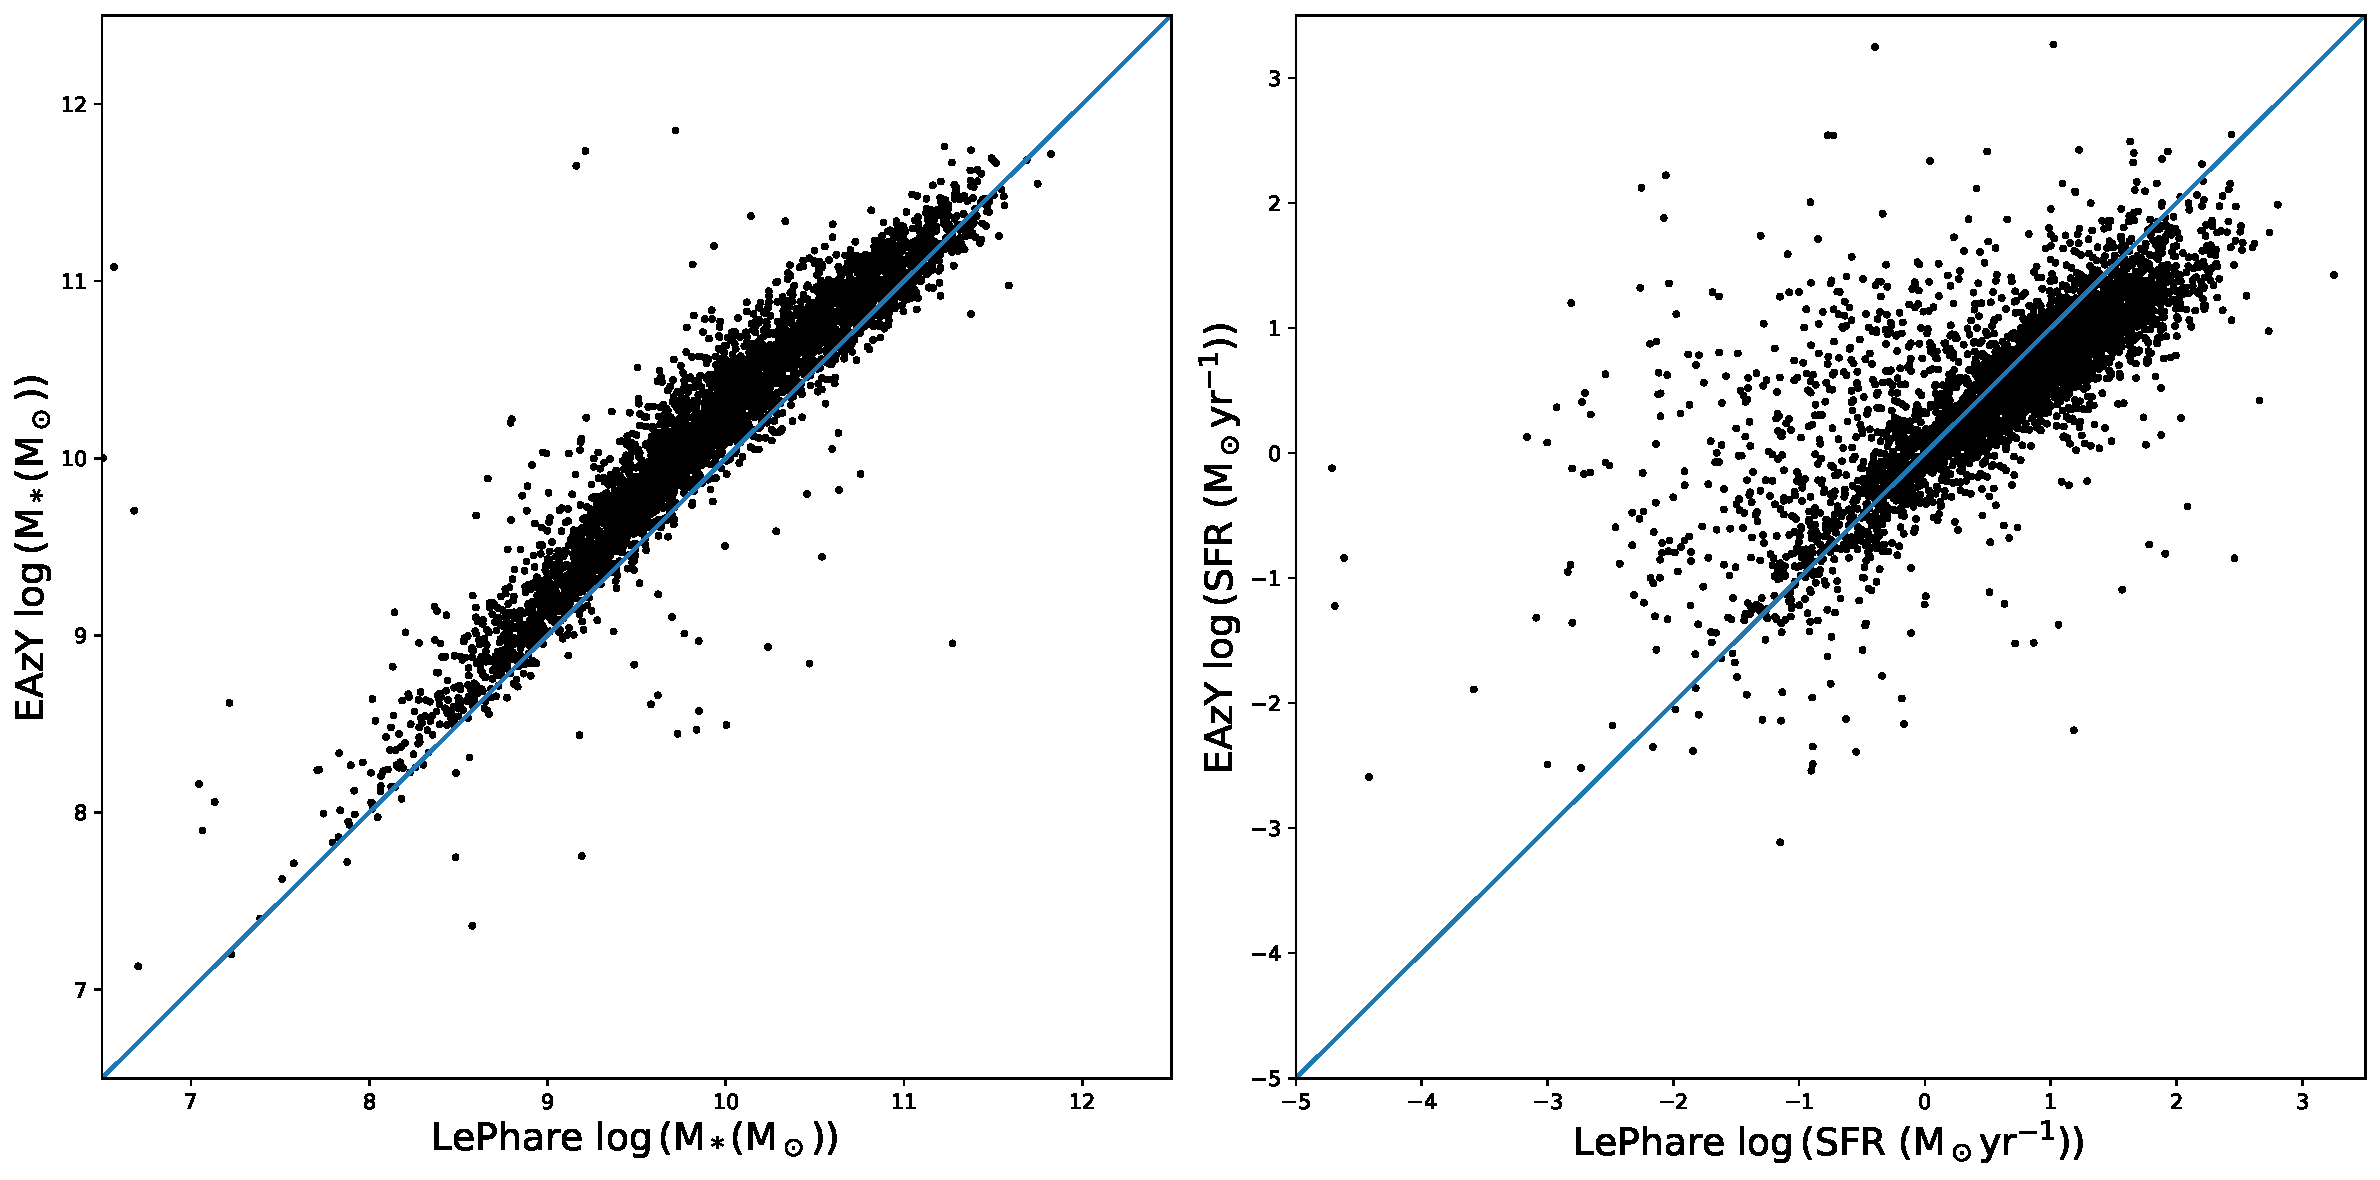
\includegraphics[width=\textwidth]{Chapter3/figures/mass-sfr-scatter.pdf}
    \caption[Comparison of the measures of stellar mass and SFR using either LePhare or EAzY/FAST photometric codes to calculate them.]{Comparison of the measures of stellar mass and SFR using either LePhare or EAzY/FAST photometric codes to calculate them. If the algorithms agreed perfectly, the sources would lie on the blue 1:1 line. \textit{Left}: The scatter in the stellar masses between softwares. As shown, EAzY often seems to find larger stellar masses when compared to LePhare. \textit{Right}: Scatter in SFRs when measured with LePhare or EAzY. There is a large difference between the measures of LePhare and EAzY here, and therefore we opt to only use EAzY measures of the SFR through this work.}
    \label{fig:difference-measures}
\end{figure}

We cross match between the catalogue of Chapter \ref{chapter2} with the COSMOS2020 catalogue by matching coordinates between them. We search the COSMOS2020 catalogue for any sources within 10" of our interacting galaxy coordinates and make a list of any COSMOS2020 sources. If more than one COSMOS2020 source is found within this radius we take the source with the smallest angular separation from the interacting galaxy coordinates as the correct source. Once we have identified one COSMSO2020 source for every ID, we de-duplicate based on COSMOS2020 ID and redo the coordinate matching process with any duplicate matches. If no further COSMOS2020 sources were within 10" of the source, then we classify the source as not in the COSMOS2020 catalogue. We find 3,786 of the our sources exist in the COSMOS2020 catalogue.

Once matched, we remove any sources with non-physical photometric measurements for the stellar mass or star formation rates. We then further reduce our sample by only keeping sources within the a mass range of $6.5 \leq \log_{10} \text{M}_{*}(\text{M}_{\odot}) \leq 12.5$ and a star formation rate range of $-5 < \log_{10} \text{SFR} (M_{\odot}yr^{-1}) \leq 3.5$. To also nullify the effect of surface brightness dimming that may occur when attempting to classify tidal features of interacting galaxies, we institute a redshift cut of $z \leq 1.2$. This also makes our sample match the catalogue that will be later used to investigate the incidence of our sample of interacting galaxies with environment (detailed in Section \ref{data:environ}). Applying these cuts reduces our sample size to 3,689 interacting galaxies.

\subsection{Secondary Identification}\label{sec:sec-ident}
\noindent As the catalogue described in Chapter \ref{chapter2} only contains source coordinates and IDs, we must also manually identify the secondaries of many of our interacting systems. To find the secondaries, we apply three steps. First, a cutout surrounding each source was created. These cutouts were from the COSMOS cutout service, selecting HST-ACS tiles in the $F814W$ filter. Each cutout had a 30" radius (corresponding to 1001 $\times$ 1001 pixels). The original cutout from Chapter \ref{chapter2} was also displayed next to the enlarged cutout. We annotate each cutout with each sources COSMOS2020 ID and measured photometric redshift and error. By annotating each cutout with the sources photometric redshift and ID, we could visually assessed each cutout and give one of four following classifications to each: system disturbed but secondary could not be identified; secondary could be identified; cannot confirm galaxy is interacting; null redshift; incorrect primary assigned. 

To classify a secondary galaxy for our primary one, it had to be within the cutout we were visually assessing and within the recorded error of the primary photometric redshift. Using photometric redshift cutoffs in this way is often done when calculating environment parameters \citep[e.g][]{2006MNRAS.373..469B} or defining interacting galaxies by close pairs \citep[e.g][]{2022ApJ...940....4S}. A null redshift is defined as one outwith our redshift limits or NaN. A minority of the cutouts we visually assessed were found to have the incorrect primary at the centre. In these cases, we record the correct primary galaxy ID and extract the ancillary data from the COSMOS2020 catalogue. We then attempt to find the secondary galaxy again for the corrected primary.

Using these definitions, we find that of the 3,689 original systems cross-matched with COSMOS2020 2,283 could not have their secondary identified, 834 had a clear secondary, 446 could not be reliably classified as an interacting galaxy, 248 had a null redshift and 149 were the incorrect primary. Figure \ref{fig:secondary_selection} shows an example of each of our classifications. Each secondary we identify was added to our sample, increasing our sample size to 3,829.

\begin{figure*}
    \centering
    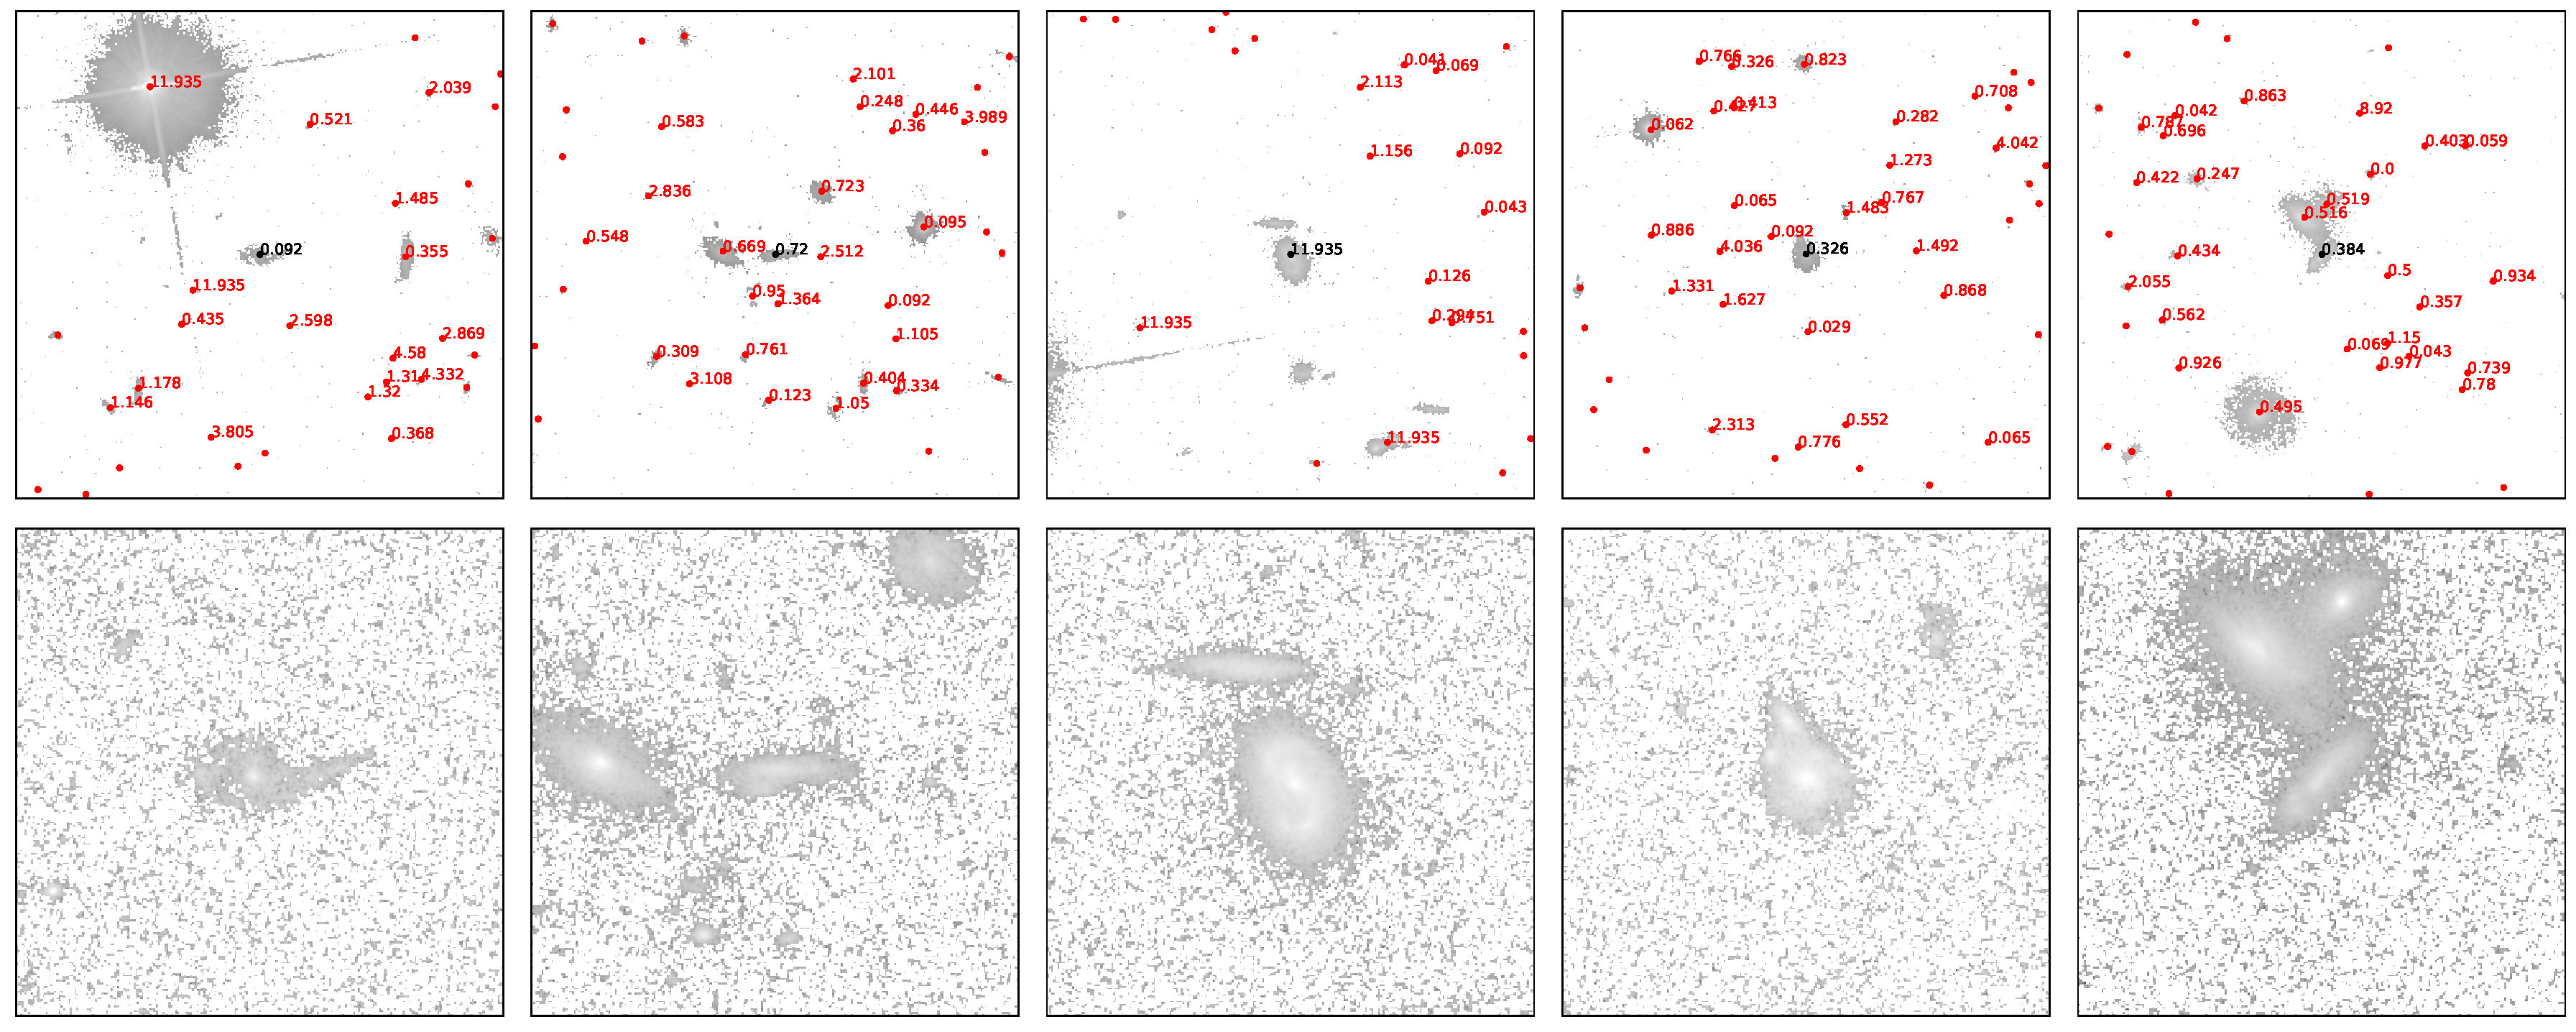
\includegraphics[width=\textwidth]{Chapter3/figures/cutouts_ex.pdf}
    \caption[An example of each visual classification made on the cross matched sample.]{An example of each visual classification made on the cross matched sample. From left to right these are: where the secondary could not be identified, the primary had a clear secondary, the primary could not be reliably classified as an interacting galaxy, the redshift was null and the incorrect primary was identified. Based on these classifications, we either add the secondary galaxies to the sample or we remove the contamination from it. These images are 30" across using the COSMOS cutout service, selecting HST/ACS tiles as the basis for the observations in the $F814W$ filter.}
    \label{fig:secondary_selection}
\end{figure*}

% Define our classifications above.
While initially surprising that the majority of our systems could not have a secondary identified, we found that it was mostly due to limitations in the COSMOS catalogue or the way in which we conduct our secondary identification. Each potential secondary must have a COSMOS ID associated with it, however, when two systems were very close together and small enough they would be identified under a single COSMOS ID despite being two separate systems. The same also occurred when two systems were merging or interacting. The tidal features connecting the systems or coalescing systems would only be identified under one ID in the catalogue. Figure \ref{fig:secondary_selection} shows an example of two systems being close enough together that they have been identified under a single COSMOS2020 entry. Figure \ref{fig:secondaries_found} shows this disparity with the different types of interaction we observe.

\begin{figure}
    \centering
    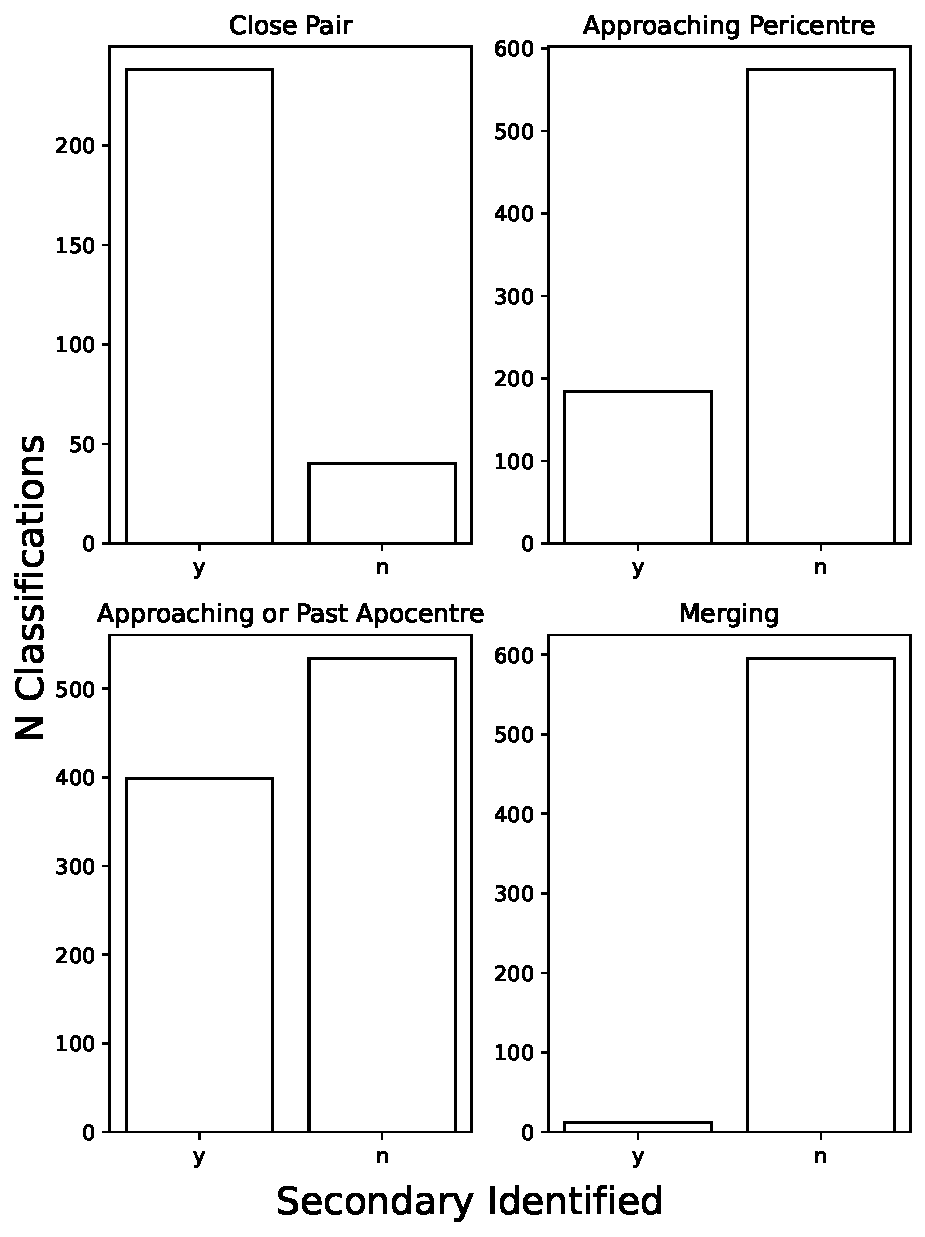
\includegraphics[width=0.95\textwidth]{Chapter3/figures/visualisation_classification.pdf}
    \caption[Where a secondary could be identified at different stages in the interaction.]{Where a secondary could be identified at different stages in the interaction. The reasoning for such disparity in secondaries identified is due to the relative distance each the secondary would be from the primary at each stage. For a close pair, we often found the secondary galaxy, but a minority of these were so close together that the entire system was given a single COSMOS ID. The same was true for those interacting systems approaching pericentre or merging. When the secondary was near apocentre, often it would be outwith the cutout we were using for visual classification.}
    \label{fig:secondaries_found}
\end{figure}

Those galaxies which were found to be contamination (i.e., could not be reliably classified as interacting or having a null redshift) were removed from our sample. Galaxies that could not be reliably classified as interacting as they showed little tidal distortion or had no neighbouring systems at a matching redshift were also removed. These systems were often overlapping but at different redshifts, or were systems with irregular morphologies of spiral arms or many clumpy galaxies. There was also many systems that were at high redshift ($z \geq 1$) where the resolution of the cutouts meant that features could not be discerned visually.

Our final classification type was that the incorrect galaxy had been identified as the priamry galaxy. This was the case for 149 systems. These were systems where the interacting galaxies were clearly in the cutout but some tidal debris or some nearby system had been cross matched from COSMOS. We reassign these systems to the correct COSMOS IDs and then take them through the secondary identification process.

By the end of this pipeline, we find a sample size of 3,829 interacting galaxies. We conduct a de-duplication based on the COSMOS2020 ID, which reduces the sample back down to 3,547 interacting galaxies. This shows that many of the secondaries we had identified for the different systems were already found in our catalogue. The remaining systems are each visually confirmed interacting and disturbed galaxies based on their morphology and photometric redshift as measured in the COSMOS2020 catalogue.

For each galaxy in our sample, we find and define a mass- and redshift-matched control galaxy to investigate differences in their galactic parameters. We find these control galaxies from the COSMOS2020 catalogue. All galaxies within 0.01 dex of our sub-samples' stellar mass are selected from the catalogue, and within a $\pm$0.01 redshift slice. We then define the control galaxy as the system furthest from our interacting galaxy. Each control galaxy is then visually confirmed to be non-interacting and have no nearby pairs. We also confirm that it does not already exist in the catalogue, and ensure there is no duplication in the control sample. Figure \ref{fig:matched-distributions} shows the mass distribution of our paired sub-sample of galaxies and their control, showing a mass distribution which is approximately the same as the interacting sample. With the previously defined cuts, we find a control galaxy for all but one of our interacting galaxies.

\begin{figure}
    \centering
    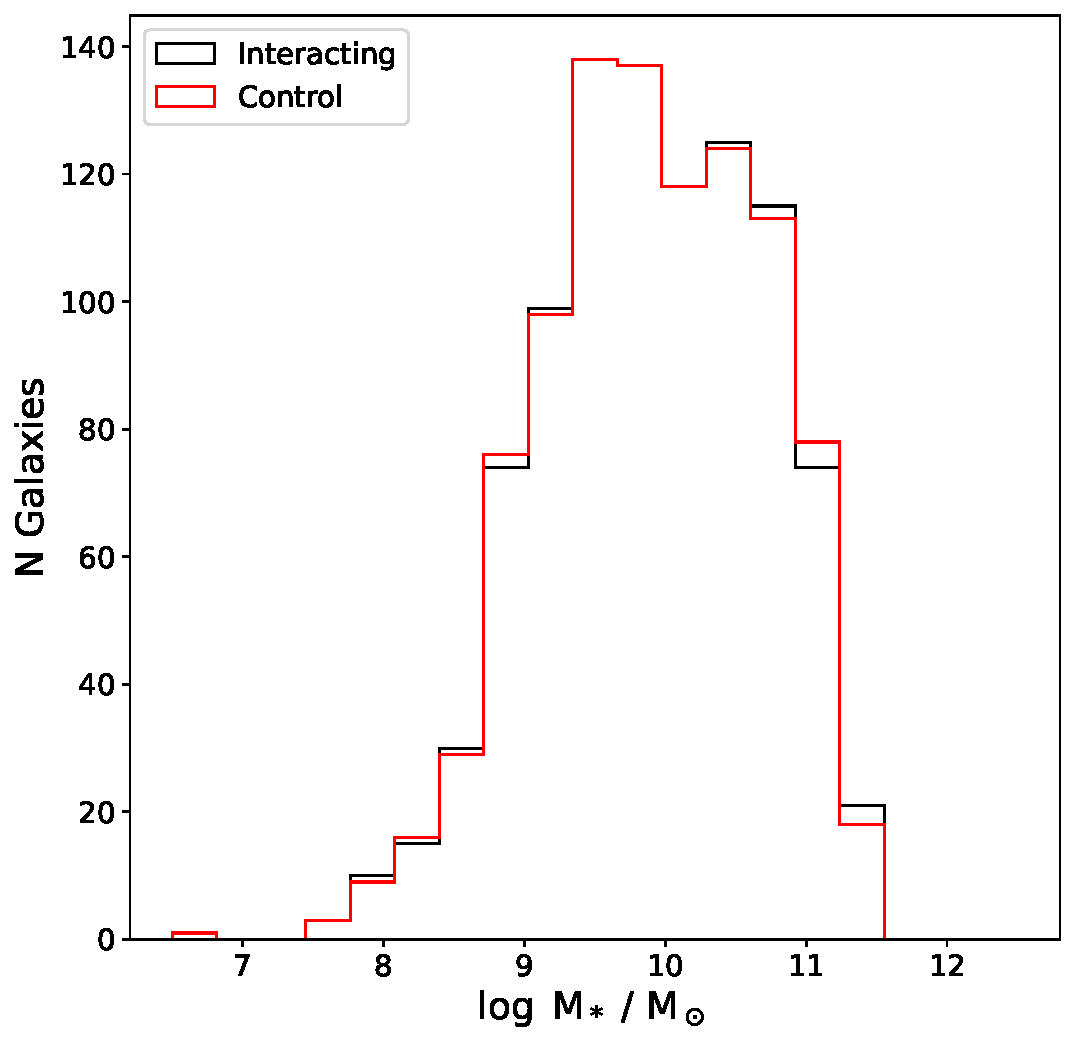
\includegraphics[width=\textwidth]{Chapter3/figures/mass-matching-pairs.pdf}
    \caption[The mass distribution of the paired interacting galaxy sample and the control sample.]{The mass distribution of the paired interacting galaxy sample and the control sample. Both primary and secondary galaxies are within this distribution. From our sample of 4,181 interacting galaxies morphologically identified, 834 are confirmed galaxy pairs. This means that the secondary in the interacting galaxy system has been identified from morphology and photometric redshifts.}
    \label{fig:matched-distributions}
\end{figure}

\subsection{Finding Additional Systems}
\noindent As a result of using visual classification to find the secondary galaxy in each interaction, we were able to also confirm other interacting systems which had not been found in our catalogue. Primarily, these extra interacting galaxies are from systems which had more than one galaxy involved in the interaction. Our pipeline was built to only find a primary and secondary galaxy and, therefore, we add these extra systems through another pipeline. Other interacting galaxies that were added were low redshift systems which would have appeared very large in the small cutouts of the classification process in Chapter \ref{chapter2}. By looking at the larger COSMOS2020 cutouts, we are able to recover these galaxies and add them to this sample.

In total, we found an extra 841 interacting systems that we could add to our sample. Upon conducting a de-duplication of these with the sample already found, this was reduced to 634 interacting systems. This gives us a total sample size of 4,181 which we use through the rest of this work.

\subsection{Redshift Effects on Visual Classification}
\noindent There are two limits when using visual morphology to find interacting galaxies. The first is the limitation of being able to characterise tidal features with increasing redshift. As the redshift increases, surface brightness dimming of the systems may lead to a lack of visual confirmation in the tidal features of different objects. Thus, if we are heavily affected by this in our redshift range ($0.0 \leq z \leq 1.2$), we would see distinct signs of it in our selection function of our mergers. For instance, if all of our stage 4 classifications were actually high redshift and high mass stage 3 galaxies, we would observe this in our selection function. Therefore, Figure \ref{fig:redshift_selection} shows our the distribution of stellar mass across our redshift range for each defined stage in our interaction. As shown, the distribution of masses across redshift that we find in our sample is reasonably consistent with each other.

\begin{figure}
    \centering
    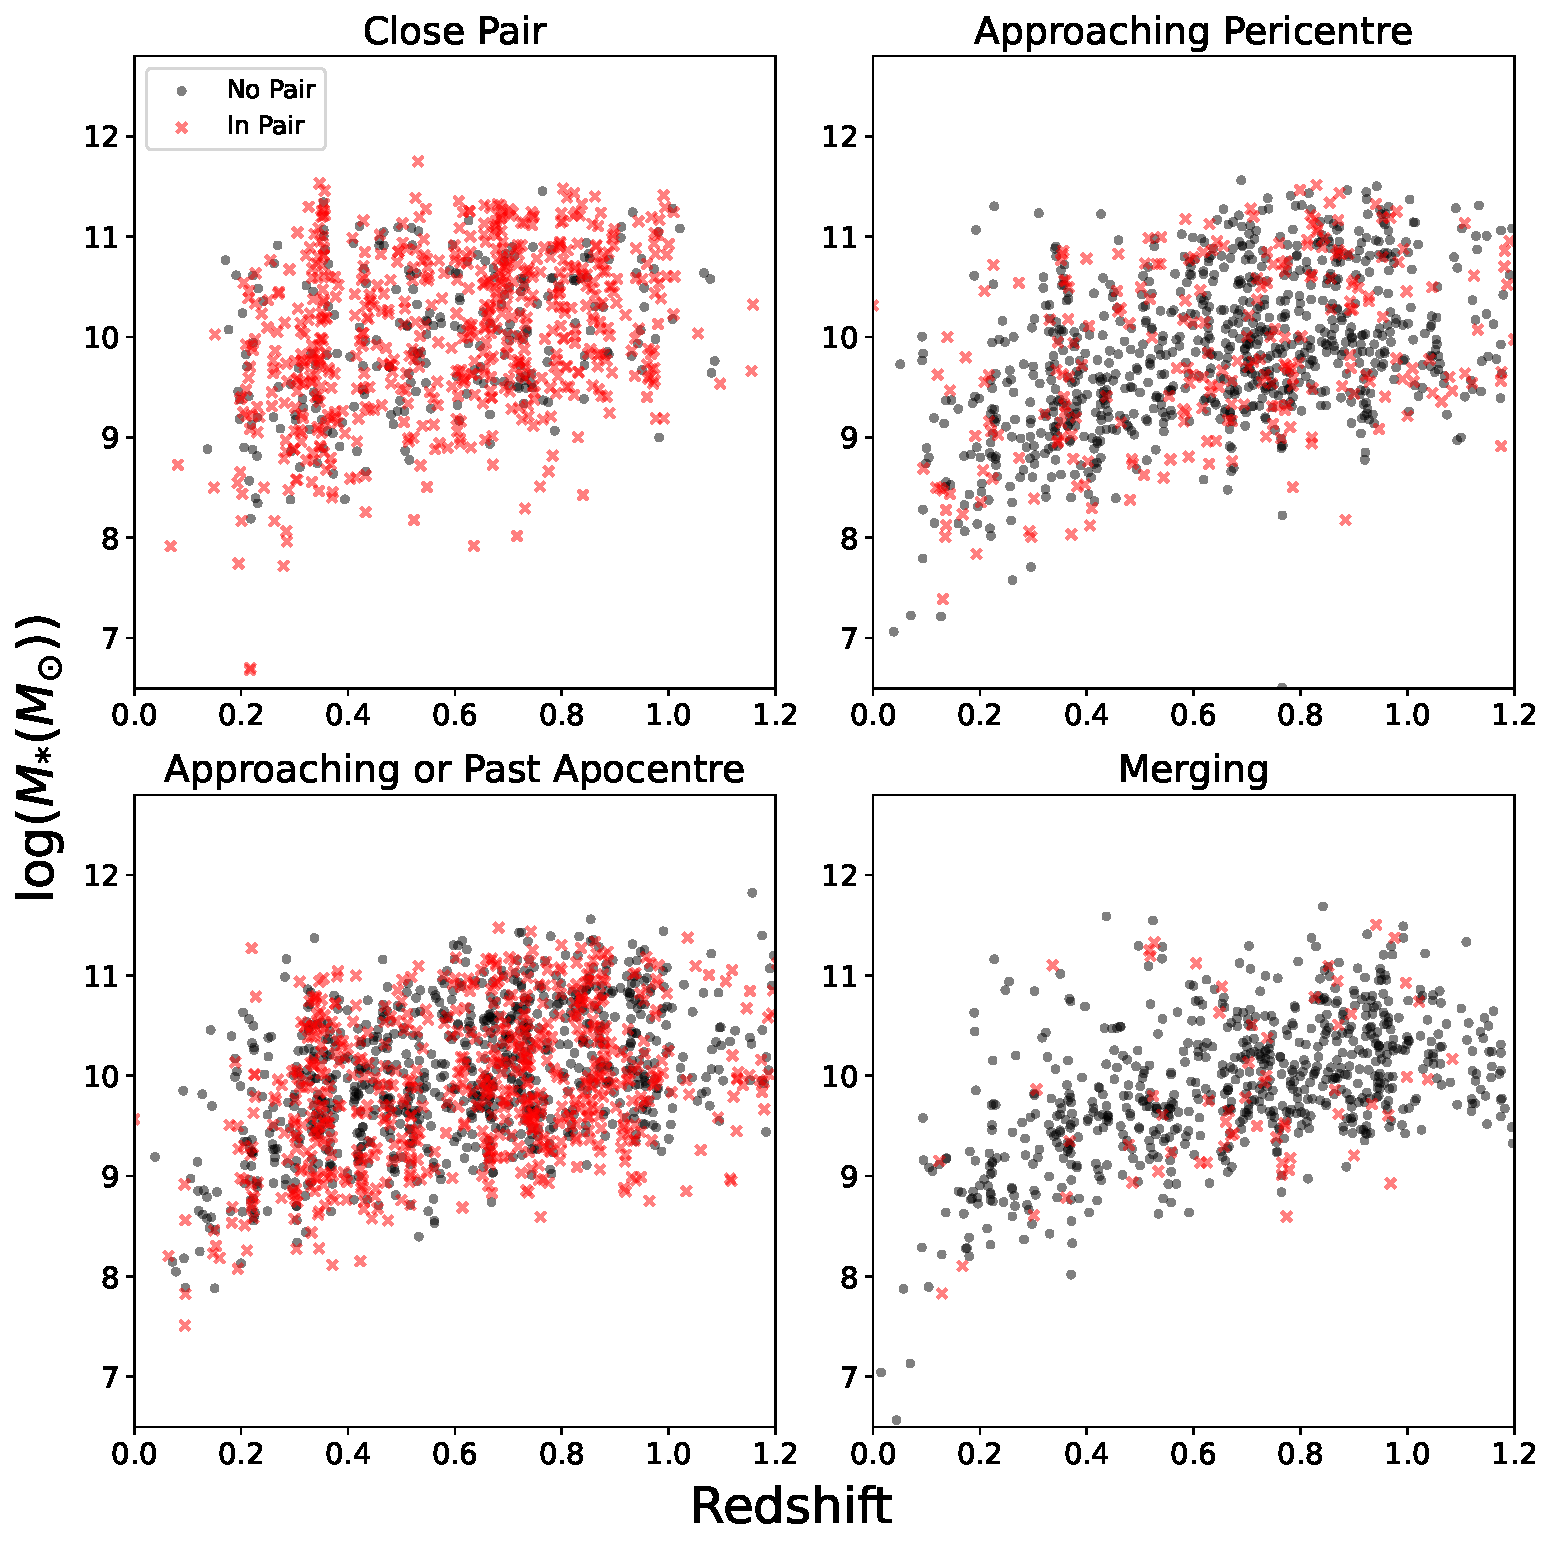
\includegraphics[width=\textwidth]{Chapter3/figures/redshift-limitations.pdf}
    \caption[Redshift vs Mass distribution for each stage of interaction we have defined.]{Redshift vs Mass distribution for each stage of interaction we have defined. This is important as we use tidal distortion and the existence as tidal features as a fundamental for our classification methodology. As shown here, the distribution of systems across redshift and mass is consistent for all stages in our sample. Therefore, we are likely not affected by this in our analysis.}
    \label{fig:redshift_selection}
\end{figure}

The second issue that could affect our sample is that of contamination by close pairs by projection effects rather than by galaxies which are physically close together. For the majority of these systems, we are limited to only having their photometric redshift from the COSMSO2020 catalogue and not their well-constrained spectroscopic redshift. As we are conducting visual classification, this issue is rather limited. The criteria on all of our sources besides stage 1 is that they must be morphologically disturbed. Each source is confirmed to have some kind of tidal feature f=present in the image, even if a secondary is not present in the image. There are, always, of course other galaxies in each image and there is no guarantee that the calculated photometric redshift is correct. We often find galaxies which are clearly interacting or paired, but with the photometric wildly different. In these cases, we defer to the redshift and only record one of the galaxies in our sample. This approach, however, means we must be careful to investigate the effects of environment on our galaxies as disturbance by, say, ram pressure stripping can appear like tidal features.

\section{METHOD: Environment, AGN and Interaction Stage} \label{method}
A primary aim of this work is to investigate the evolution of different galactic parameters with stage of the interaction. Each stage is defined to capture a different part of the dynamical time and merger history. This stage also relates to the projected separation of galaxies with an identified secondary. Here, we fully define what we mean by interaction stage and which part of the dynamical time it covers. We also describe how we find AGN in our full sample and find measurements of the environment about each. The parameters required to calculate the AGN fraction are not found in the COSMOS2020, and we therefore must cross match with other catalogues to find the required parameters. We also describe the catalogue we use to define the environmental density about each of our sources. This is important to consider, as it is well known that measured SFRs of galaxies can be affected by environment, as well as existing biases in where interacting and merging galaxies reside. We, therefore, need to check that we have not introduced any environmental biases into our definition of interaction stage. 

\subsection{Classifying Stage of Interaction}\label{sec:staging}
The primary goal of this work is to find if a relation exists between a host of galactic parameters, underlying physical processes and the stage of the interaction. Each stage covers a different part of the dynamical history in an interaction and, in this case, we define it based on the morphology and projected separation between systems. We define four distinct stages of interaction:

\begin{itemize}
    \item Stage 1: Systems which are well-separated with little to no morphological disturbance (Close pairs).
    \item Stage 2: Close pairs showing morphological distortion while still in a pair or show a physical connection by tidal features.
    \item Stage 3: Well separated pairs with morphological disturbance or isolated galaxies with clear tidal features.
    \item Stage 4: Highly disturbed systems with two or more cores within them.
\end{itemize}

\noindent Figure \ref{fig:stages} shows the original source cutouts used in Chapter \ref{chapter2} to give an example of each stage. There are degeneracy's associated with this staging system, however. In this context, we define a degeneracy as when the interacting galaxies may be at two or more parts of the dynamical timescale and we have no way to tell without further information on the system.

\begin{figure}
    \centering
    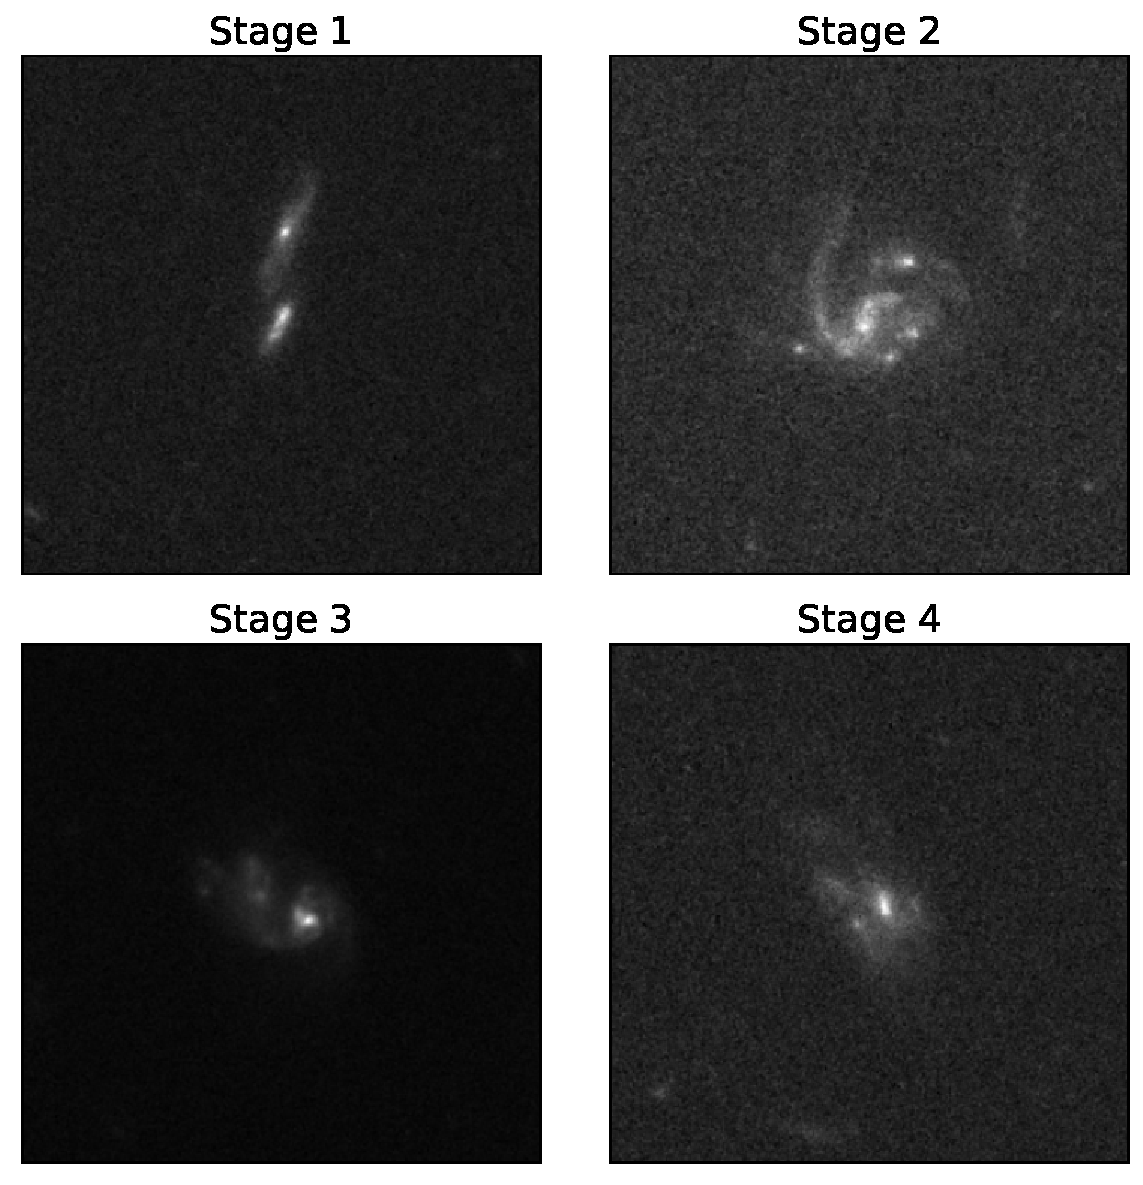
\includegraphics[width=\textwidth]{Chapter3/figures/examples-stages.pdf}
    \caption[Examples of the four stages we split our interacting galaxy sample into.]{Examples of the four stages we split our interacting galaxy sample into. Stage 1: A close pair with confirmed redshift matching. Stage 2: Two distinct systems interacting with tidal features forming. Stage 3: A tidally disturbed system with no secondary present, likely at apocentre. Stage 4: A galaxy with multiple cores while highly disturbed. At the final stage before coalescence.}
    \label{fig:stages}
\end{figure}

\begin{figure*}
    \centering
    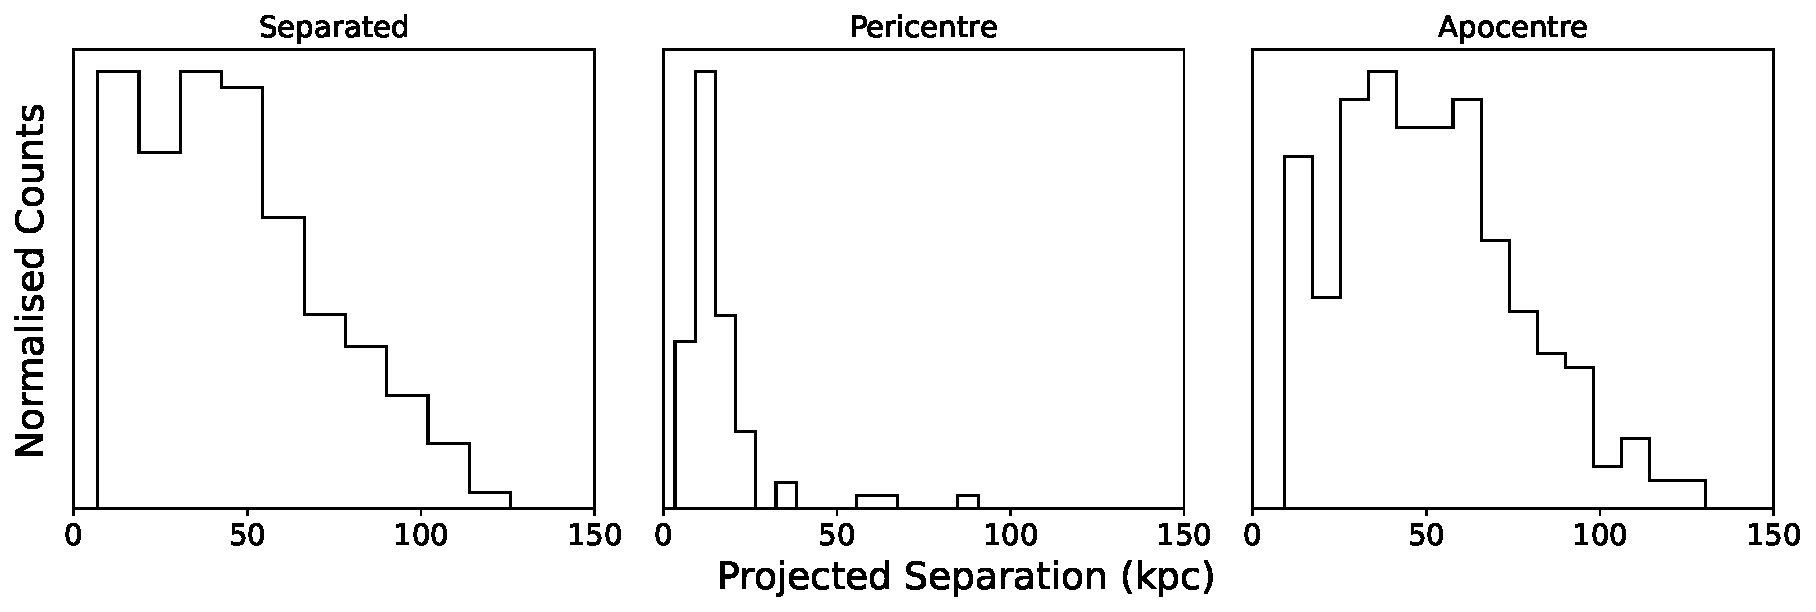
\includegraphics[width=\textwidth]{Chapter3/figures/projected-seps.pdf}
    \caption[The projected separations of the confirmed galaxy pairs in our sample.]{The projected separations of the confirmed galaxy pairs in our sample. This confers with other works the definition of our different stages. Stage 1 can be at any projected separation, however, we have visually confirmed that these sources are not morphologically disturbed. Stage 2 is dominated by systems with small projected separation as, by definition, they must be morphologically linked or overlapping. Those systems at larger separation are very large systems whose morphology categorise them as stage 2. Finally, stage 3 galaxies are those which are visually confirmed to be fully morphologically separated and tidally disturbed. The bulk of these lie in a range of 25 - 100kpc in projected separation from each other. There is some overlap between stage 2 and stage 3 in projected separation, as their visual classification is also dependent on the system size.}
    \label{fig:proj-seps}
\end{figure*}

Stage 1 of the interaction captures the first approach of the two systems and they are observed as a galactic pair. They have no morphological disturbance yet and, in our sample, are most often those galaxies with distinct disks. At this point, we would expect no change in the underlying processes of the galaxies from their control samples. Interaction has not taken place yet, and the two systems are morphologically intact. By definition, this stage requires an identified secondary galaxy and therefore has the highest number of identified secondaries with every system having a secondary that can be visually classified. This is also the least degenerate part of the dynamical time we are sampling due to a criteria being no morphological disturbance. Therefore, it is unlikely that the galaxies would have already flown by each other.

Stage 2 of the interaction is defined as the point where the two galaxies in the interaction are are at or just passing the pericentre of the tidal encounter. At this point, we find the beginning of morphological disturbance, the beginning of the formation of tidal features and some tidal debris. Due to the two systems having to overlap or connect via tidal features - by definition - this is the stge that suffers most from limited identification of the secondary galaxy. The COSMOS2020 catalogue often defines these two systems as a single system, and therefore, we lack information about their secondary. This stage is also highly degenerate in the context of the dynamical timescale of the interaction. Without further information, we are unable to define whether the galaxies involved at this stage are at the first, second, third, etc passage of the tidal encounter. We also do not know if they are just passing pericentre on the first pass, or if they are approaching pericentre on more than one pass.

Stage 3 describes those interacting systems where the two disks are fully separated and distinct from one another. They must have some morphological disturbance associated with them, but do not require a secondary galaxy to be put into this stage as if the galaxies have sufficient velocity they would escape from each other and, therefore, their secondary could be outwith our COSMOS2020 cutouts used to visually identify them. This is reflected in an even distribution of finding the primary and secondary in this stage. This stage is also defines a large part of the dynamical timescale. It spans from separating from the secondary and after pericentre, to moving out to the apocentre of the interaction (or escaping with sufficient velocity), to falling back in towards the secondary galaxy again. Without velocity information, we have no way of finding if the galaxy is moving away or moving towards its secondary.

Finally, stage 4 represents the final step of a galaxy interaction. If the two galaxies do not have sufficient velocity to escape one another, then they go on to coalesce and ultimately merge. We define this stage through the severe morphological disturbance of the galaxy involved as well as the existence of a second core within it. While we attempt to capture only pre- or ongoing-coalescing systems, it is important to note that this stage is degenerate to post-merger remnants which will also be accepted by our criteria. Post-merger remnants are systems where coalescence has been completed and immediately after will be highly morphologically disturbed and difficult to distinguish from those systems with merging ongoing. At this stage, we would expect the interaction will be at its most violent with complete disruption of both galactic disks and likely increased star formation across the disk. 

Our four stage approach is not a new one, and many other works have utilised it to differentiate different parts of the dynamical history of a galaxy interaction \citep{2022ApJ...937...97C, 2023ApJ...952..122G}. We have noted the degeneracy of each stage as we have described them. Thus, we can now put this fully into the context of the dynamical timescale. Over a typical interaction, we would expect the galaxy pair to always move from stage 1 to stage 2 in the early times of the dynamical timescale. Then, dependent on the velocity of the system, the galaxy pair will either move straight into stage 4 of classification and begin to merge or it will move into stage 3. This change from stage 2 into stage 3 can then take many branching paths dependent on the velocity in the system. If the galaxies have sufficient velocity, stage 3 will be their end state until the tidal features slowly dissipate. If they do not have velocity to escape on another, the system will move from stage 3 back into stage 2. This could then happen for many cycles until finally the galaxies enter stage 4 and coalesce. Figure \ref{fig:illustration} shows the branching paths that the galaxies can take through each stage. Note, these are created using the Advanced Python Stellar Animation Module restricted numerical simulation \citep[][O'Ryan et al., in prep.]{2016A&C....16...26W} and are for illustrative purposes only.

\begin{figure*}
    \centering
    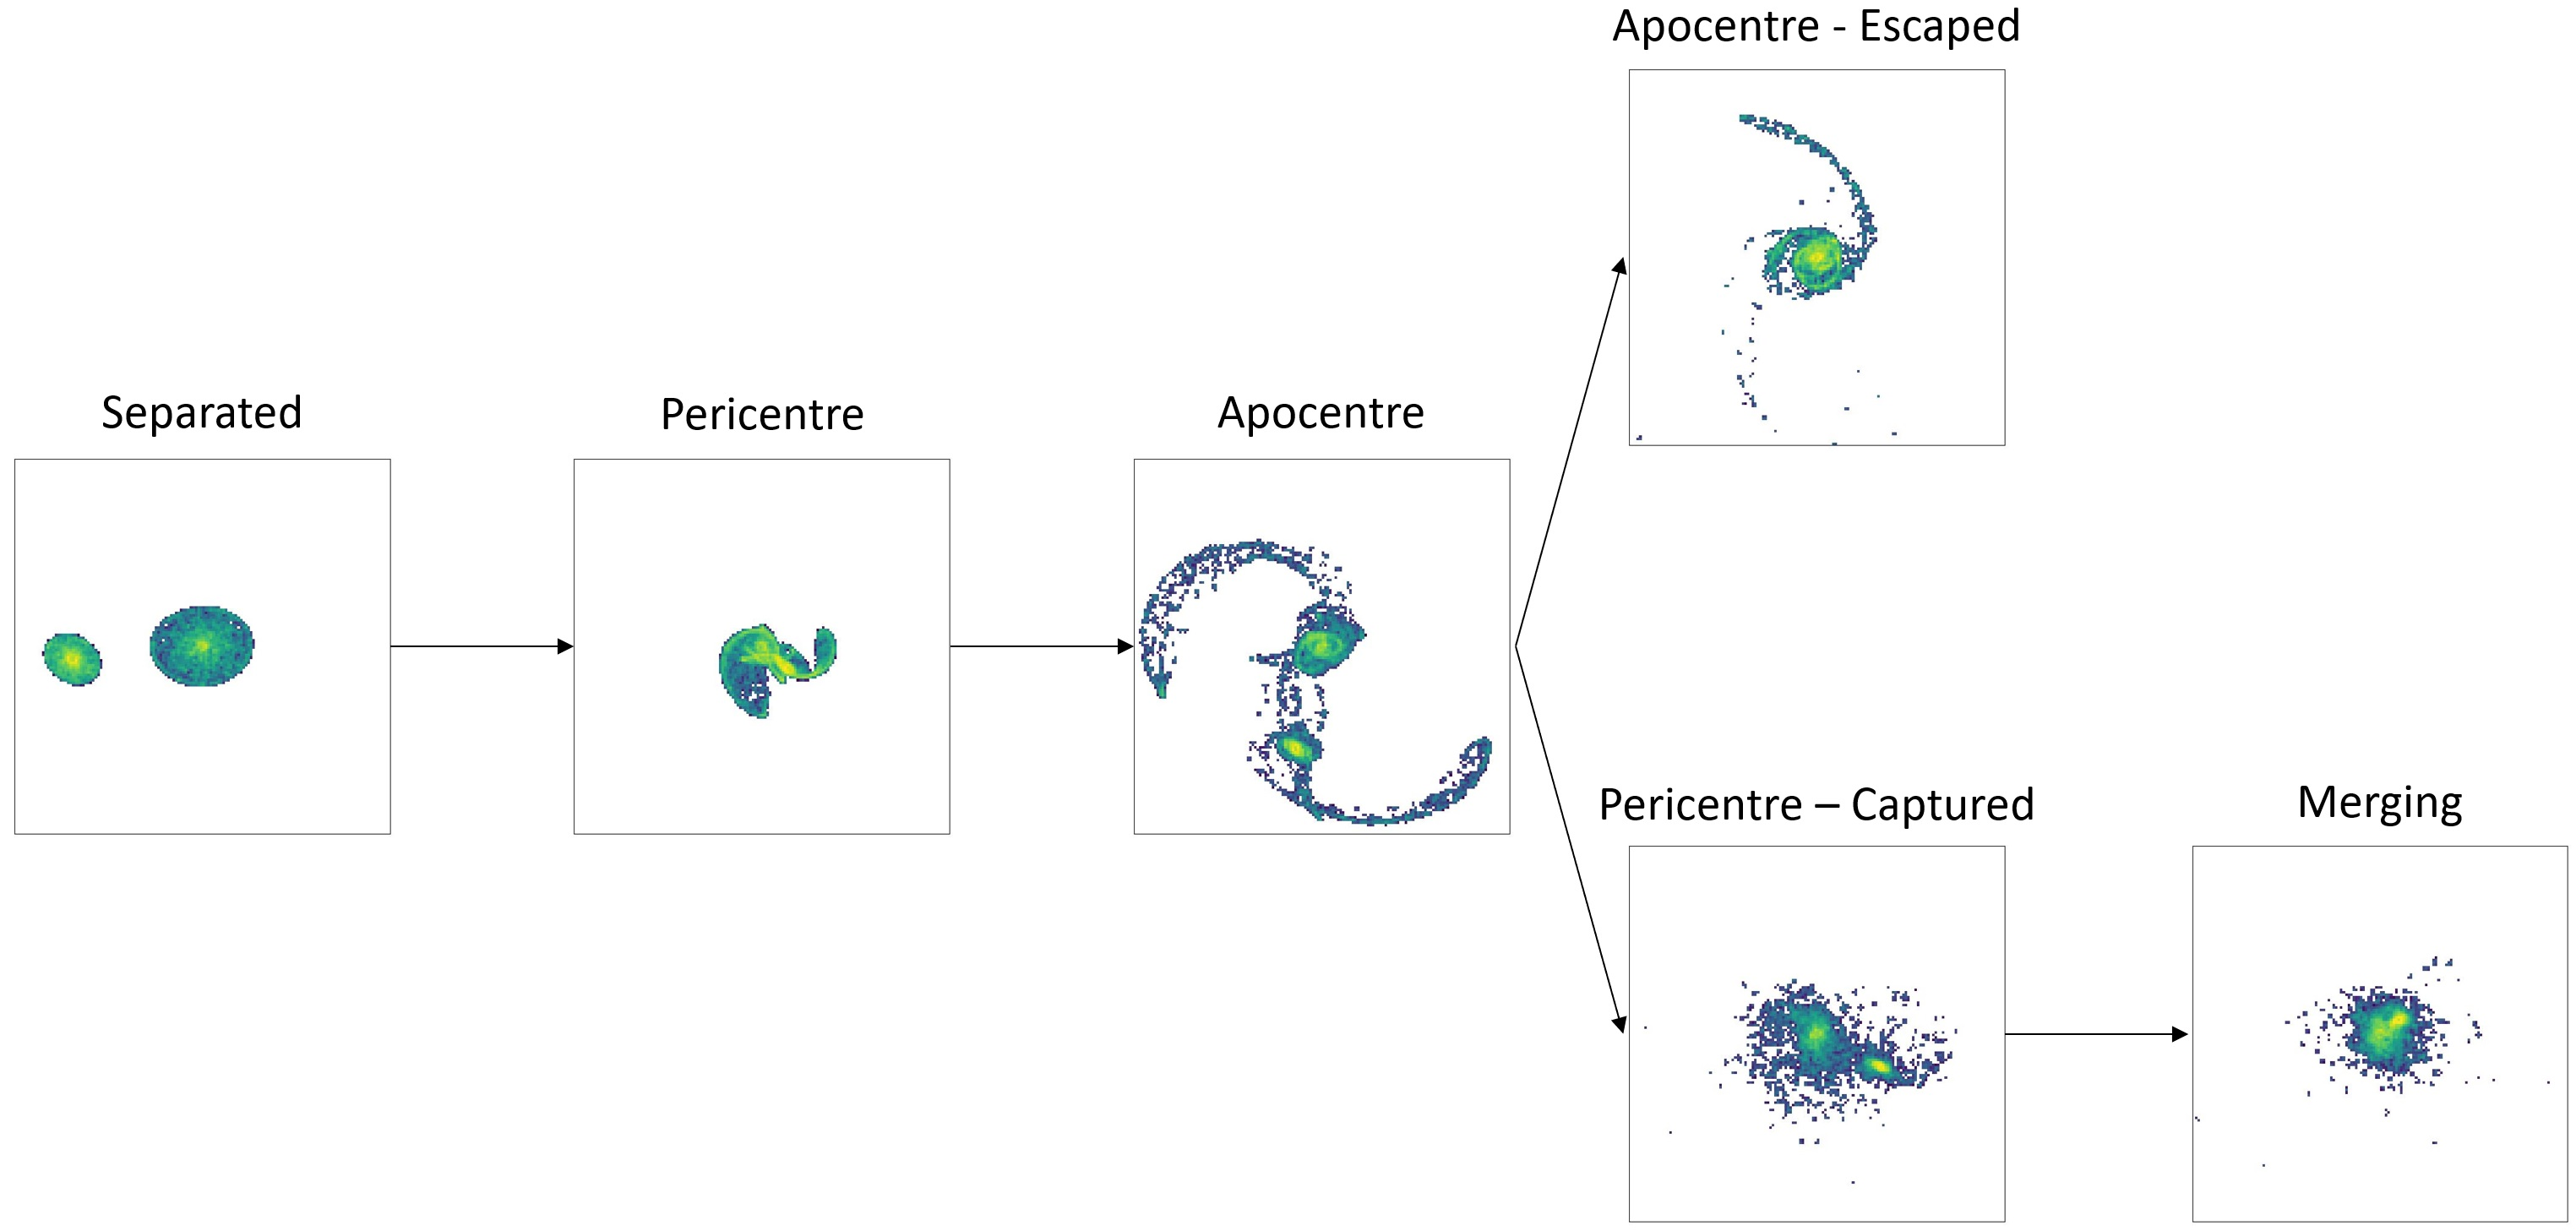
\includegraphics[width=\textwidth]{Chapter3/figures/stage-evolution.jpg}
    \caption[The progression through an interaction using our stage definitions.]{The progression through an interaction using our stage definitions. In stage 1, we have two systems that are approaching each other but exhibit no tidal features. This is before the point of closest approach has occurred. This is followed by an intial stage 2: the systems are approximately at their closest approach. This stage is often mistaken, in the COSMOS catalogue, for being of only one source. Clear tidal features exist with major disturbance in the two disks. This is followed by stage 3, where there are two distinct cores with clear tidal features. However, after this point, there are two outcomes to the system depending on the galactic velocities. If the secondary has the escape velocity, the system will remain a stage 3 interaction until the tidal features dissipate (and no longer are in our sample). If they do not have enough energy, the system will return to stage 2 of the encounter and then begin to merge at stage 4. Images are from the Advanced Python Stellar Particle Annimation Module interacting galaxy algorithm described in O'Ryan et al. (in prep.) and based on the stellar particle animation module algorithm described in \citet{2016A&C....16...26W}.}
    \label{fig:illustration}
\end{figure*}

More commonly, in the literature, rather than using the stage of an interaction based on morphology we use the projected separation of the two systems. To explore the difference between using our staging system and the projected separation, as well as to ensure we recover the expected relations, we measure the projected separations of our confirmed galaxy pairs. Figure \ref{fig:proj-seps} shows the stage classification with projected separation between the two pairs. We measure this by taking the average of the best fit photometric redshifts between the two galaxies, and converting their angular separation to a physical one. The most distinct projected separation ($s_{proj}$) in stages is between stage 2 and stage 3. Here, we see that stage 2 is dominated by systems with $s_{proj}<$35kpc while stage 3 is dominated $25 \leq s_{proj} \leq 100$ kpc. Stage 2 is visually classified as systems which are highly morphologically disturbed, while either being morphologically linked to each other or overlapping. Those galaxy pairs with large projected separations are pairs which are very large in angular size, while still overlapping or morphologically linked. If this criteria is not met, then the system becomes a stage 3 interaction where the two galaxies in the pair are completely distinct. There is some overlap between the projected separations of stage 2 and stage 3 as this is somewhat dependent on the angular size of the two systems involved in the interaction. 

We will use the projected separation to investigate relations between AGN activity and if we observe enhancement in star formation with stage. The SFR is already present in the COSMOS2020 catalogue from both EAzY/FAST and LePhare. To ensure that any enhancements are from interaction alone, we must ensure we have no bias' in the environment distribution of our sample and identify AGN. We, therefore, cross match to two further catalogues COSMOS catalogues containing the required information.

\subsection{Matching to Environment Catalogue}\label{data:environ}
\noindent There is no measure of the environmental density in the COSMOS2020 catalogue. Such a measure is often calculated in numerous ways, such as the N-nearest neighbour \citep{2006MNRAS.373..469B}, different Bayesian metrics \citep{2008ApJ...674L..13C} or estimating it from Voronoi Tesselation \citep{2021inas.book...57V}. However, in this work, we utilise the existing environmental density catalogue produced by \citet{2017ApJ...837...16D}. This catalogue was created specifically for the COSMOS survey, and has a measured density for all sources with mass $\log(\frac{M}{M_\odot}) \geq 9.6$ and $z \leq 1.2$. \citet{2017ApJ...837...16D} calculate not only the density, but also the density parameter $\delta$ and assign each source to a field, filament or cluster classification. For a full description of how they calculate the environment and density field see \citet{2015ApJ...805..121D} and \citet{2017ApJ...837...16D}, but we will briefly describe it here.

To build the density field throughout the COSMOS field, \citet{2017ApJ...837...16D} first construct a set of overlapping redshift slices. Within each slice, a subset of the galaxies are selected such that the median of the probability distribution function (PDF) of their photometric redshift is within it. Then, from this subset, they calculate the weighted surface density within the redshift slice. The weighting is based upon the PDF of the photmetric redshift present within the redshift slice. These weights significantly reduce the effects of projection effects. They then apply a weighted adaptive kernel smoothing using a 2D Gaussian kernel whose width changes based on the found local density of galaxies. Once this density field is created, the density around the sample galaxies can simply be interpolated across the density field based on the angular position and the redshift slice the sample galaxy is in (based on its photometric redshift PDF).

The result of this process, and the cuts defined previously, is a catalogue of $\approx$45,000 galaxies with their densities accurately measured. We remove any sources which are flagged as uncertain from the catalogue (a flag existing within it) providing us with $\approx$39,000 sources with which to cross match the sample from Chapter \ref{chapter2}. We apply the same cuts to our sample as applied in \citet{2017ApJ...837...16D}, and only consider those systems with a mass $\log(\frac{M}{M_\odot}) \geq 9.6$. To cross match with our sample, we simply utilise the COSMOS2015\_ID which exists in both the COSMOS2020 catalogue and the \citet{2017ApJ...837...16D} catalogue. Upon applying the mass cut to our sample, we find that we are matching 2,800 sources to the \citet{2017ApJ...837...16D} catalogue. Upon matching based upon the COSMOS2015 ID, we find that 628 sources in our sample do not exist in the environment catalogue. This reduces our sample to 2,172 galaxies with confirmed and reliable environment density measurements.

\subsection{Classifying AGN}\label{sec:agn-clsf}
\noindent We will also investigate the effect of interaction stage on AGN activity throughout our sample. As the COSMOS2020 catalogue does not contain the relevant parameters to make this calculation, we turn to the Chandra COSMOS Legacy Survey Multiwavelength Catalogue \citep{2016ApJ...817...34M} and the COSMOS VLA 3GHz survey \citep{2017A&A...602A...6S, 2017A&A...602A...3D}. Both of these catalogues span the entire COSMOS area, and contain detailed classifications of the sources they find. The Chandra survey spans the X-ray range of wavelengths, and successfully identified numerous X-ray AGN. The VLA 3GHz survey is a radio survey, and we use this to find the radio AGN through our sample. 

Our cross match process is very much the same as previously described. We use the previously identified COSMOS2020 source coordinates and conduct a radial search of 10". If more than one source is within this radius, we match on the closest source. We first find matches of radio AGN using the VLA 3GHz survey catalogue and then search the Chandra survey. At every step, if we find a match in the relevant catalogue, we remove it from subsequent searches in other catalogues and take the first classification as the correct one.

Applying our matching criteria, we find 1,059 classifications in the VLA 3GHz survey and 155 in the Chandra survey. These were split into 812 star forming galaxies and 402 AGN. We also investigate cross matching with the MPA-JHU catalogue \citep{2003MNRAS.341...33K, 2004MNRAS.351.1151B, 2007ApJS..173..267S}, however, found that all matches were already represented by the VLA and Chandra surveys. We also utilise the COSMOS XMM-survey and, again, find no new sources to add to our sample. While the ratio of AGN to star forming galaxies in our sample seems large compared to other works, it is important to note that this is a result of limited matching between the catalogues. Of the 4,181 galaxies in our sample, only 1,214 appeared at all in either the VLA or Chandra catalogues. Any galaxy which did not appear in these catalogues, we discard as unclassified. 

\section{STAR FORMATION EVOLUTION WITH INTERACTION STAGE}\label{results:SF_stage}
\subsection{Controlling for Interaction Stage}
\noindent With the above samples selected, we investigate the change in multiple parameters with stage of the interaction. The four stages of interaction are designed to capture the main different parts of galaxy interaction. First, we show the results of breaking down our sample into stages with relation to the star formation and mass of our sample. We utilise the estimates of these parameters that exist in the COSMOS2020 catalogue itself. Then, we utilise our subsample of galaxy pairs to recover the relationship between projected separation and star formation enhancement (SFE). We then further break this measure down into its component stages.

Figure \ref{fig:sfr-mass} shows the breakdown of stellar mass and SFR with stage. On a population scale, there is clear evolution in the star formation rate from stage 1 through to stage 4. In stage 1, where the galaxies are distinct from one another with no clear morphological disturbance, we clearly see two populations of galaxies. These are the blue, star-forming galaxies and red sequence of galaxies. The blue contours in Figure \ref{fig:sfr-mass} show increasing number density in the population into the blue cloud. In stage 2, when the galaxies are actively interacting and overlapping, this red sequence remains but is highly diminished while there is no change in the blue cloud. Stage 3 shows a similar effect, where the red sequence reduces again before finally in stage 4 the red sequence completely disappears. Through these, the blue cloud remains highly populated and hosts the majority of galaxies in the sample.

\begin{figure}
    \centering
    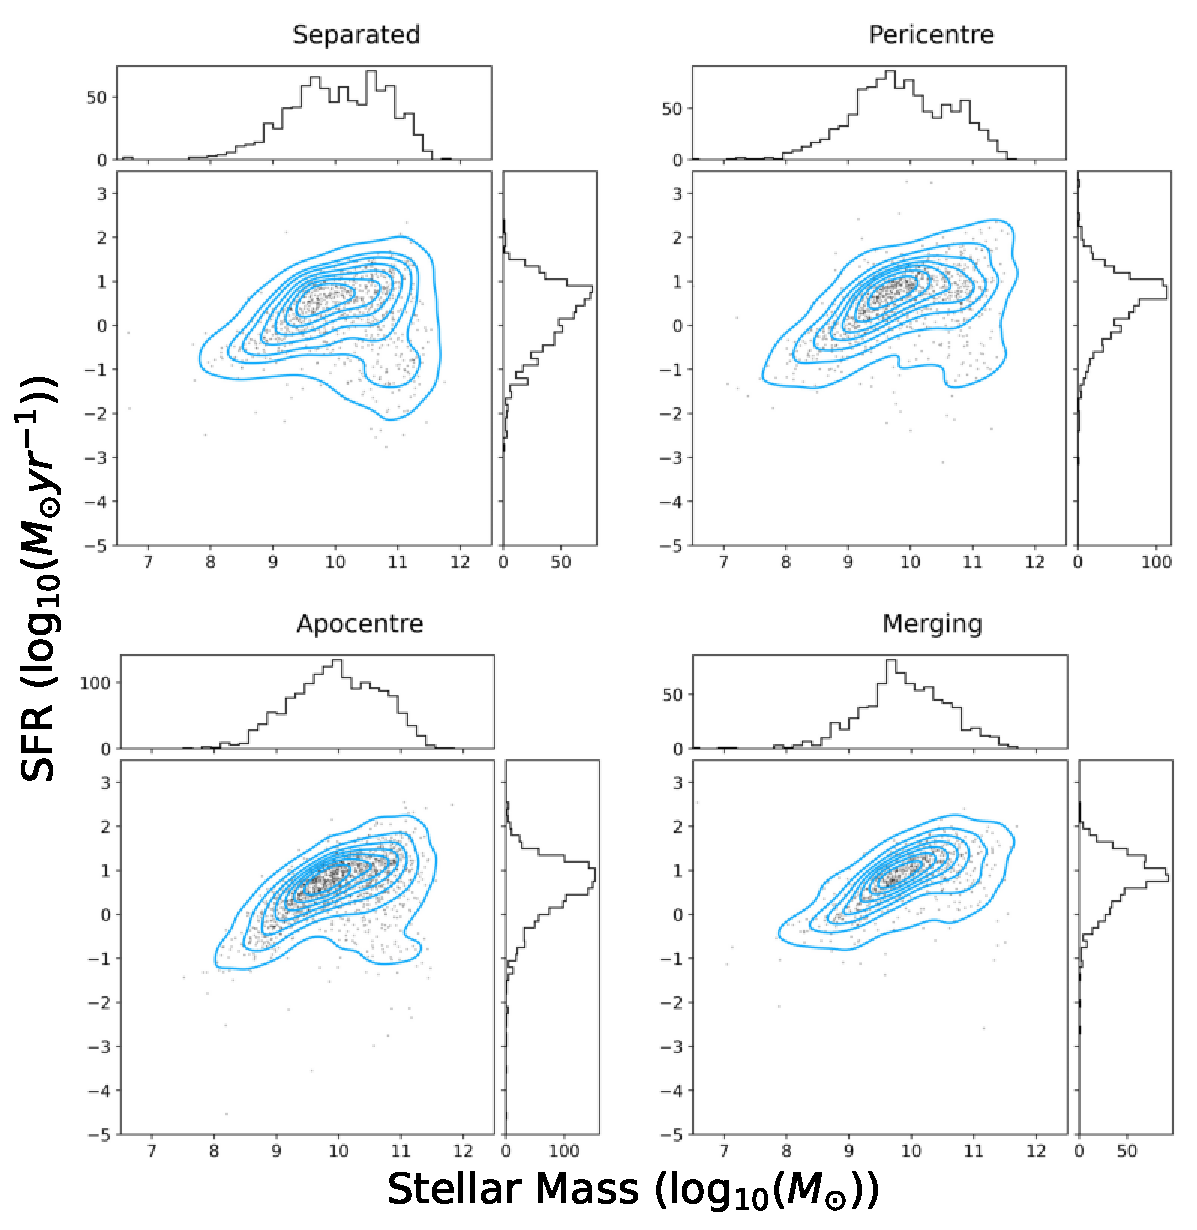
\includegraphics[width = \textwidth]{Chapter3/figures/sfr-mass-stages.pdf}
    \caption[The LePhare stellar mass against the EAzY SFR across the different stages of the interaction.]{The LePhare stellar mass against the EAzY SFR across the different stages of the interaction. The blue contours are 8 levels of density of the underlying populations in each frame. \textit{Top left}: The stellar mass and star formation rate of Stage 1 of our sample. Here, the interacting galaxies are simply close pairs with little to no morphological disturbance. There are clearly two populations here: a main, star forming sequence forming the main population and a smaller red sequence. \textit{Top right}: Stage 2 of the interaction, where the two interactors are close to pericentre. The star forming sequence remains, but the red sequence is reduced significantly. \textit{Bottom left}: Stage 3 of the interaction, where the interactors are close to apocentre or escaped. Here, we see the almost complete disappearance of the red sequence. \textit{Bottom Right}: Stage 4 of the interaction, where the two systems are close to coalescence or have merged. The red sequence of galaxies has completely disappeared.}
    \label{fig:sfr-mass}
\end{figure}

However, this result could also be due to many other factors rather due to interaction stage. For instance, if the mass distribution of our sources evolves as well, we could simply be selecting higher mass systems as we increase stage. This would have the result of systems in stage 4 having, on average, higher SFRs than those in stage 1 and appearing like we had evolution in the star forming population with stage. Another effect that could cause this relation to appear would be our selection was highly dependent on galactic environment. It is well known that environment and star formation are closely linked, and that classifying interacting galaxies by morphology classifiers can weight up galaxies in cluster environments over galaxies in the field. In Section \ref{sec:env-cont}, we control for the environment in our sample and show that this is not the case. Here, we investigate the question of the evolution of the mass distribution that could give us this result.

We can quantify the similarity of the mass distributions, and then the SFR distributions, using well known statistical tests. We opt to use two different tests: the Kolmogorov-Smirnov \citep[KS-test;][]{an1933sulla} and Anderson-Darling \citep[AD-test;][]{stephens_74}. The KS-test is excellent at comparing different weighted distributions and indicating if they are drawn from the same parent sample. The AD test tests for this similarity as well, and we utilise both to ensure consistency and robustness in our measurements. First, we create weighted distributions of stellar mass. The weighting scheme we utilise balances the distributions such that each bin could be assumed to have the same number of sources within it. Therefore, any bins with fewer than a certain number of sources will be weighted up while those bins with more will be weighted down. These weights applied to the mass distribution are then applied to the SFR distribution as to control for stellar mass in this distribution.

\begin{figure}
    \centering
    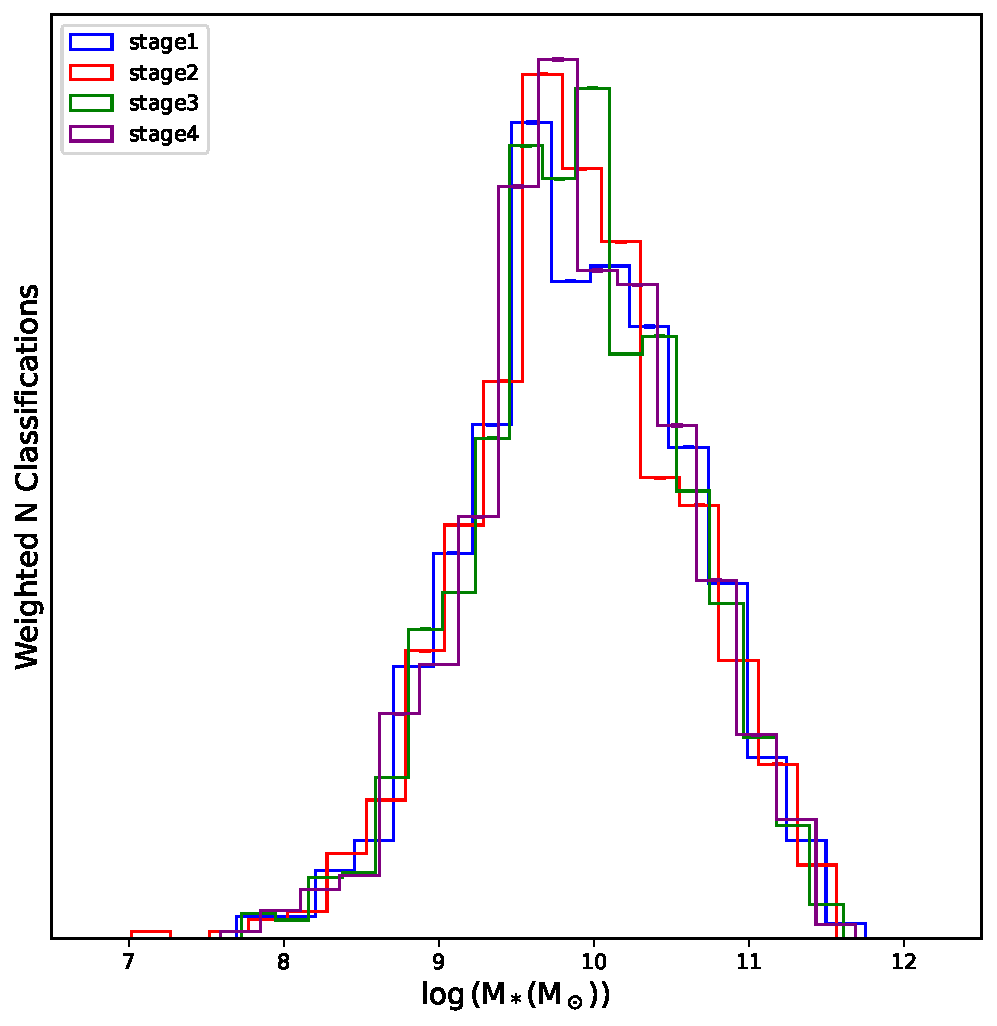
\includegraphics[width = \textwidth]{Chapter3/figures/stellar-mass-dist.pdf}
    \caption[The stellar mass distribution across the four stages.]{The stellar mass distribution across the four stages. Each bin is weighted based on the counts in the smallest sub-sample in stage. This is stage 4 of interaction.}
    \label{fig:weighted-mass}
\end{figure}

\begin{figure}
    \centering
    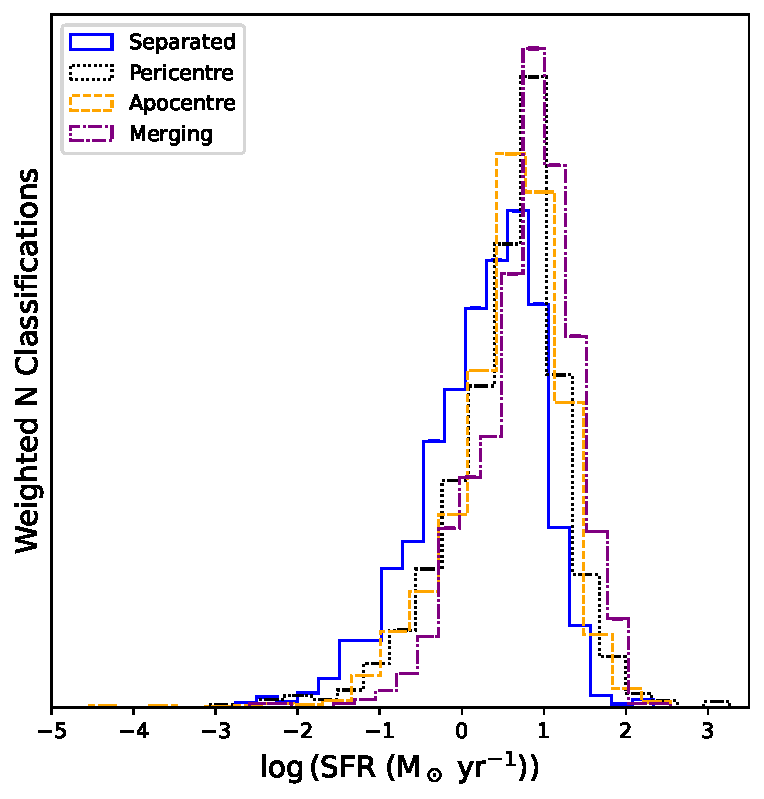
\includegraphics[width=\textwidth]{Chapter3/figures/sfr_dist.pdf}
    \caption[SFR distribution weighted by mass across each stage.]{SFR distribution weighted by mass across each stage. This weighting is based on our sample of stage 4.}
    \label{fig:weighted-sfr}
\end{figure}

Figure \ref{fig:weighted-mass} shows the weighted mass distributions through the four different stages. These appear highly similar, however to statistically measure the similarity we apply our KS- and AD-tests to them. We chain the KS- and AD- test through each distribution and calculate the value of the test values and a p-value. This p-value represents the probability that each distribution is drawn from the same parent distribution. For each mass distribution, we find that p-value of both tests is approximately one. Thus, proving that the distribution ins tellar mass though each stage is very similar, and no stellar mass evolution is occurring. Figure \ref{fig:weighted-sfr} shows the SFR distributions while being weighted by stellar mass. When comparing stages 1 and 2, 1 and 3, 1 and 4, 2 and 4 and 3 and 4, the p-values are $\ll$0.05. This allows us to reject the null hypothesis for these distributions and assume they are from different parent samples and are very disimilar. However, for comparing stages 2 and 3, the p-value of the KS test is $\approx$0.90. Thus, while these distributions are likely to be not identical, they are very similar in the parent sample they have been drawn from. \textbf{For the same mass distribution through each stage of interaction, the star formation distribution radically changes from stage 1 to stage 2 and from stage 3 to stage 4, while remaining reasonably similar from stage 2 to stage 3.}

Putting this result into the context of the dynamical timescale of an interaction, it shows there are distinct points at which the SFR changes in these systems. The first is when the interacting system moves from being a close pair to actually morphologically disturbing each other in a close flyby. This difference, most likely enhancement, then persists through through to stage 3 - where the galaxies remain highly disturbed but are no longer overlapping with their secondary. The SFR distribution remains approximately the same between these two, meaning the forces that drive and affect star formation remain equivalent between these two stages. Finally, the SFR radically changes again when we approach the merging or post-merger stage of the interaction. We can also say that this change is likely an enhancement in the SFR of the galaxies through the interaction due this change being driven by the disappearance of the red sequence through each stage.

We further examine this result by controlling for redshift and making specific classification of galaxy type. While the red sequence is significantly reduced across across each stage, it is difficult to ascertain the change in the galaxies within the blue cloud. We expect that, due to an interaction, the population of starbursting and quiescent galaxies will change. Therefore, we define a star forming main sequence (SFMS) through across redshift. This allows us to classify each source based on its SFR independently of redshift. To define the star forming main sequence, we follow the example of \citet{2019MNRAS.484.4360A}. There, they define the star forming main sequence as a function of galactic stellar mass and redshift as

\begin{equation}
    \log \text{SFR}_{\text{MS}}(z)[M_\odot yr^{-1}] = -7.6 + 0.76\log\frac{M_*}{M_\odot} + 2.95\log(1+z).
\end{equation}

\noindent This finds the expected, main sequence, SFR of a galaxy at a given stellar mass, $M_*$, and redshift, z.

The ratio of the measured galaxy SFR and the expected main sequence SFR is then taken. We then use this fraction to classify each galaxy into distinct bins. These are:

\begin{enumerate}[(i)]
    \item Starburst galaxies. Here, the galaxy SFR is highly elevated compared to the SFMS. We follow \citet{2019MNRAS.484.4360A} and define a cutoff of $\log$SFR/SFR$_{\text{MS}} >$ 0.4.
    \item Main sequence galaxy. The galaxy is within 0.4 dex of the SFMS and approximately has the expected SFR. Defined as $-0.4 < \log$SFR/SFR$_{\text{MS}} < 0.4$.
    \item Sub-main sequence galaxy. A galaxy whose SFR is below the majority of the SFMS, but likely not quiescent. Defined as $-1.3 < \log$SFR/SFR $_{\text{MS}} < $ -0.4.
    \item Quiescent (High) galaxy. A galaxy with an SFR in the top $\approx$50\% of the quiscent galaxy population. Defined as $-2.3 < \log$SFR/SFR $_{\text{MS}} <$ -1.3.
    \item Quiescent (Low) galaxy. A galaxy with low SFR and very likely completely quenched. Defined as $\log$SFR/SFR $_{\text{MS}} <$ -2.3.
\end{enumerate}

\noindent We split our sample into its different stages and apply these criteria. Figure \ref{fig:sfr-clsf} shows the ratio between the expected SFMS SFR and the measured SFR in the COSMOS2020. This clearly shows a large increase in galaxies classified as starburst from stages 1 to 4 and a large reduction in the number of quenched systems. Figure \ref{fig:sfr-clsf-bar} shows the change in fraction of the different galaxy classifications through stage, reflecting the results found in Figure \ref{fig:sfr-mass}. Initially, in stage 1, we find that the majority of our galaxies lie on the SFMS or just below it. There also exists a small population of galaxies which are classified as starburst with a population of quiescent galaxies that is roughly double the starburst fraction. As we move through the interaction stage, we see that the quiescent galaxy fraction gradually decreases to the point of almost non-existence in stage 4 galaxies. The complete inverse is true in our starburst fraction. We find that this almost quadruples in the fraction of our sample over the course of the different stages of interaction. The fraction of galaxies on the SFMS remains dominant throughout, however, we do find the fraction of sub-MS galaxies significantly reduced. Thus, we find that, in general, the SFR of these galaxies is increasing with interaction stage (though, not in stage 2 - 3), but not hugely. It appears to have sub-MS and quiescent galaxies move up and join the SFMS (as it remains dominant). But, many galaxies from the SFMS are moved upwards and into a starbursting phase.

\begin{figure}
    \centering
    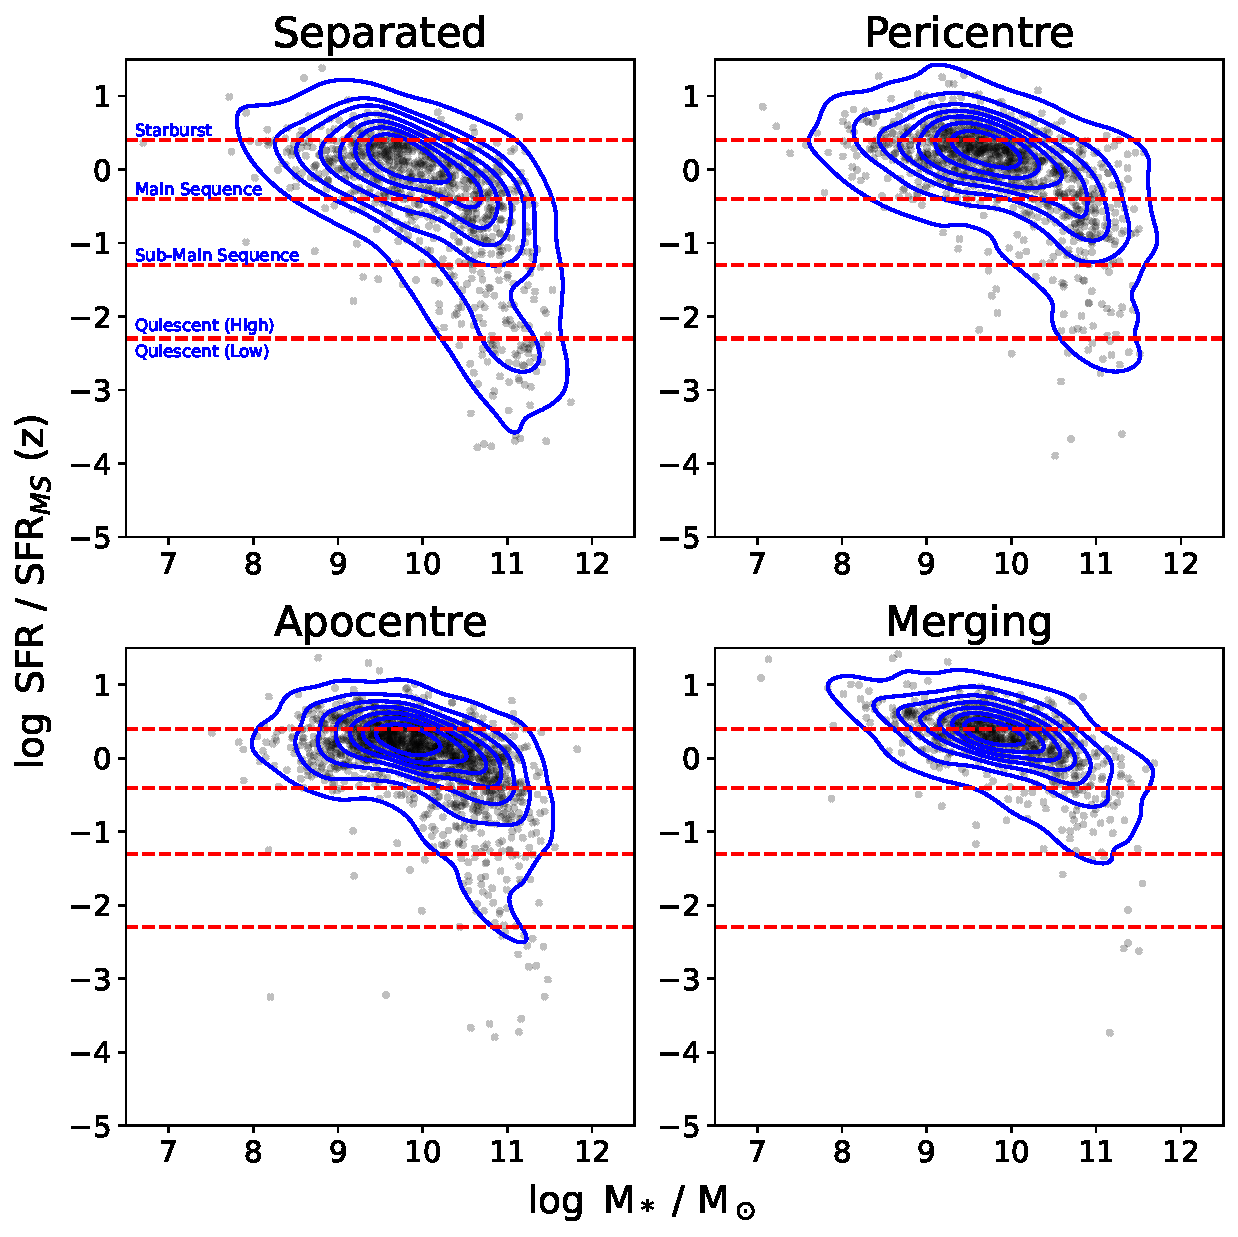
\includegraphics[width=\textwidth]{Chapter3/figures/sfr-clsf-dist.pdf}
    \caption[Stellar mass against the ratio of measured SFR to the expected SFR if the galaxy was on the SFMS.]{Stellar mass against the ratio of measured SFR to the expected SFR if the galaxy was on the SFMS. Black points are the individual sources, while the blue contours are as in Figure \ref{fig:sfr-mass}. The red dotted lines show the cutoffs for different galaxy classifications based on their SFR, with each cut off being defined by the text in blue. We find that through interaction stage, the quiescent galaxy population significantly reduces while the starburst population rapidly increases. As these cutoffs are also dependent on redshift, we find that this evolution in SFR with interaction stage is independent of redshift.}
    \label{fig:sfr-clsf}
\end{figure}

\begin{figure}
    \centering
    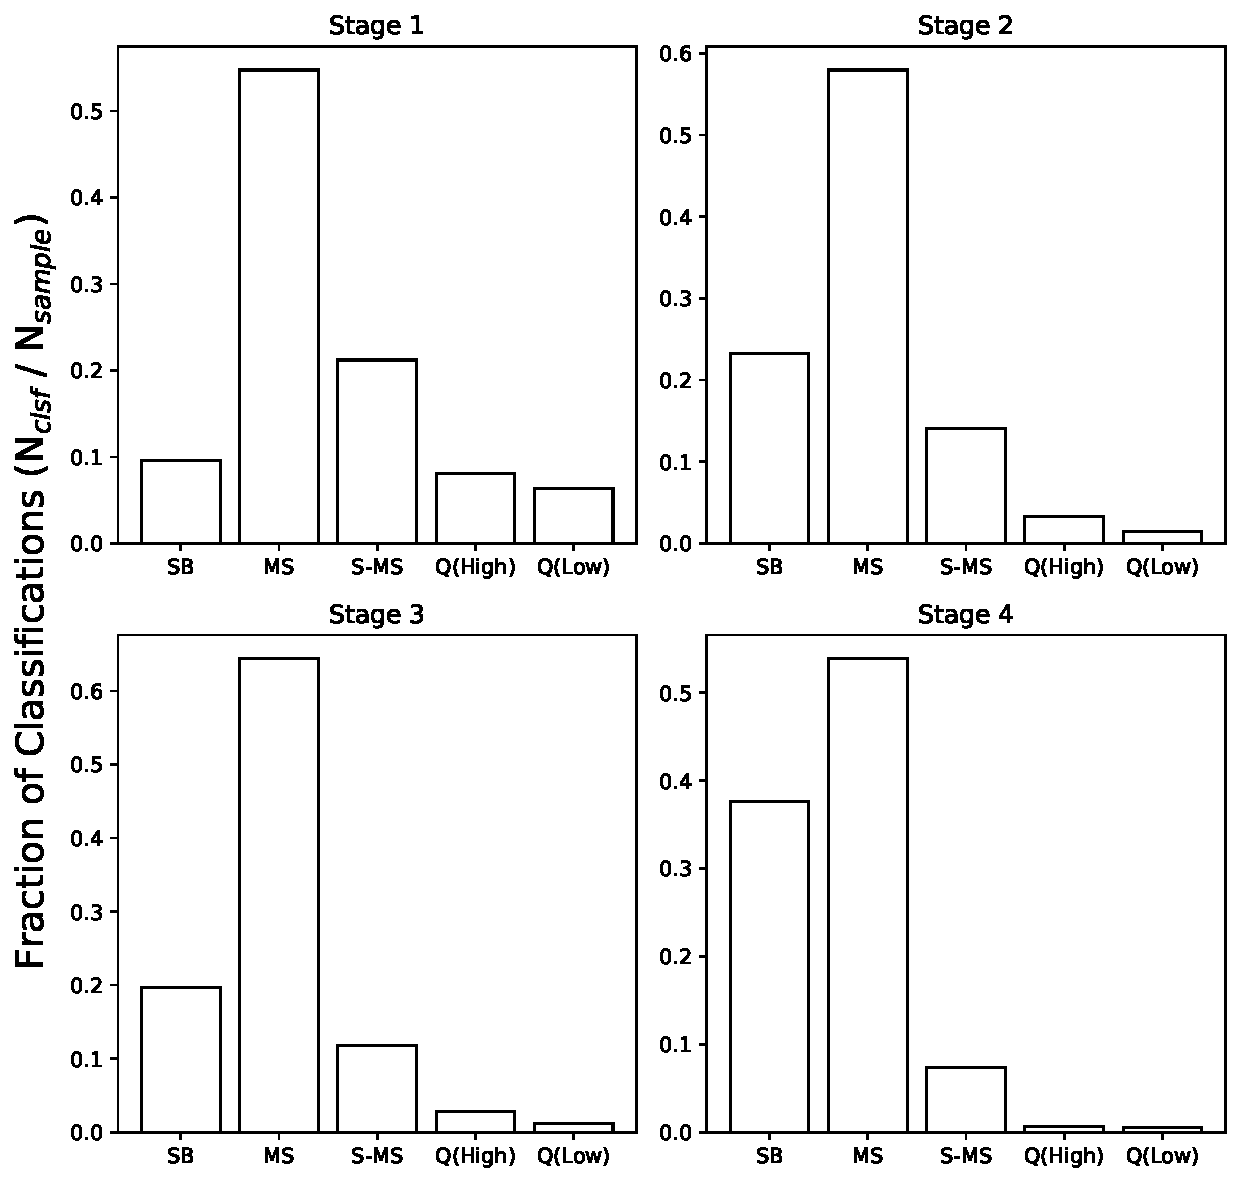
\includegraphics[width=\textwidth]{Chapter3/figures/sfr-clsf-bar.pdf}
    \caption[The change in fraction of different galaxy classifications from the fraction of SFR to the expected SFR on the SFMS.]{The change in fraction of different galaxy classifications from the fraction of SFR to the expected SFR on the SFMS. While galaxies on the SFMS remain dominant through each sample across interaction stage, there is significant change in the starburst and quiescent populations. The starburst galaxy population moves from being roughly half the size of the quiescent population in stage 1 to completely dominating it in stage 4. This is occurring while the quiescent population is significantly reduced to almost non-existence in stage 4.}
    \label{fig:sfr-clsf-bar}
\end{figure}

Now, it is important to note the parameter space that we are searching in these examples. We are probing interactions between galaxies of high mass, where the resultant tidal features that form would be classifiable in an image. Hence, even those mergers which are considered dry - with very little gas - would be capable of driving major rejuvenation in the star formation of these systems. However, we do not see a significant increase in the starbursting population until we the two galaxies begin to actually coalesce. However, \textbf{we find clear, statistically robust evolution of a galaxys' SFR with interaction stage. The SFR changes dramatically from stage 1 to 2 and stage 3 to 4 - after the initial passage of closest approach and at the point of coalescence of the interaction.}

\subsection{Projected Separation and Star Formation Enhancement}
\noindent We directly investigate the relation between the star formation enhancement (SFE) and the projected separation using our confirmed sub-sample of galaxy pairs. This sample is significantly smaller than our non-pair sample: containing 480 pairs or 960 galaxies (we have also added some pairs from the additional interacting galaxy sample). Upon sub-dividing this into different stages we find 310 stage 1 galaxies, 146 stage 2 galaxies and 498 stage 3 galaxies. Only 3 stage 4 galaxies were in our confirmed galaxy pair sub-sample, and therefore we do not attempt to make inferences about this population. 

To measure the SFE of our galaxy pairs, we directly compare to the mass- and redshift-matched control sample that was also created with this sub-sample and defined in Section \ref{sec:sec-ident}. We separate our galaxy pairs into different bins based on the projected separation between them. We find that the bulk of our sample has a projected separation between the two galaxies of $\leq$50kpc. Therefore, we sample from this region of the parameter space with high precision and smaller bin widths before we increase the bin widths at larger projected separations. We define a cutoff that each bin must contain at least 10 counts to be included in this plot and, therefore, by changing the bin widths with projected separation we are able to maintain some level of statistical robustness. We define our bins as [0.5, 10, 20, 50, 100, 125, 150] kpc.

We create two projected separation distributions: one of interacting galaxies and the other of our control galaxies. We then take the average of each bin. By taking the average of each bin, we find the total excess of the SFR caused by interaction alone and then comparing it to what we would expect from non-interacting galaxies in the same bin. Note, that the control galaxy relation to the projected separation is meaningless as they are not paired. The control galaxies are simply mass and redshift matched to each interacting galaxy and used as a reference for what SFR we would expect of it had it not been interacting. Finally, we divide the the averaged interacting SFR distribution by the averaged control SFR distribution. This provides us with a measure of the excess star formation due to interaction, and the SFE when compared to the regular population.

\begin{figure*}
    \centering
    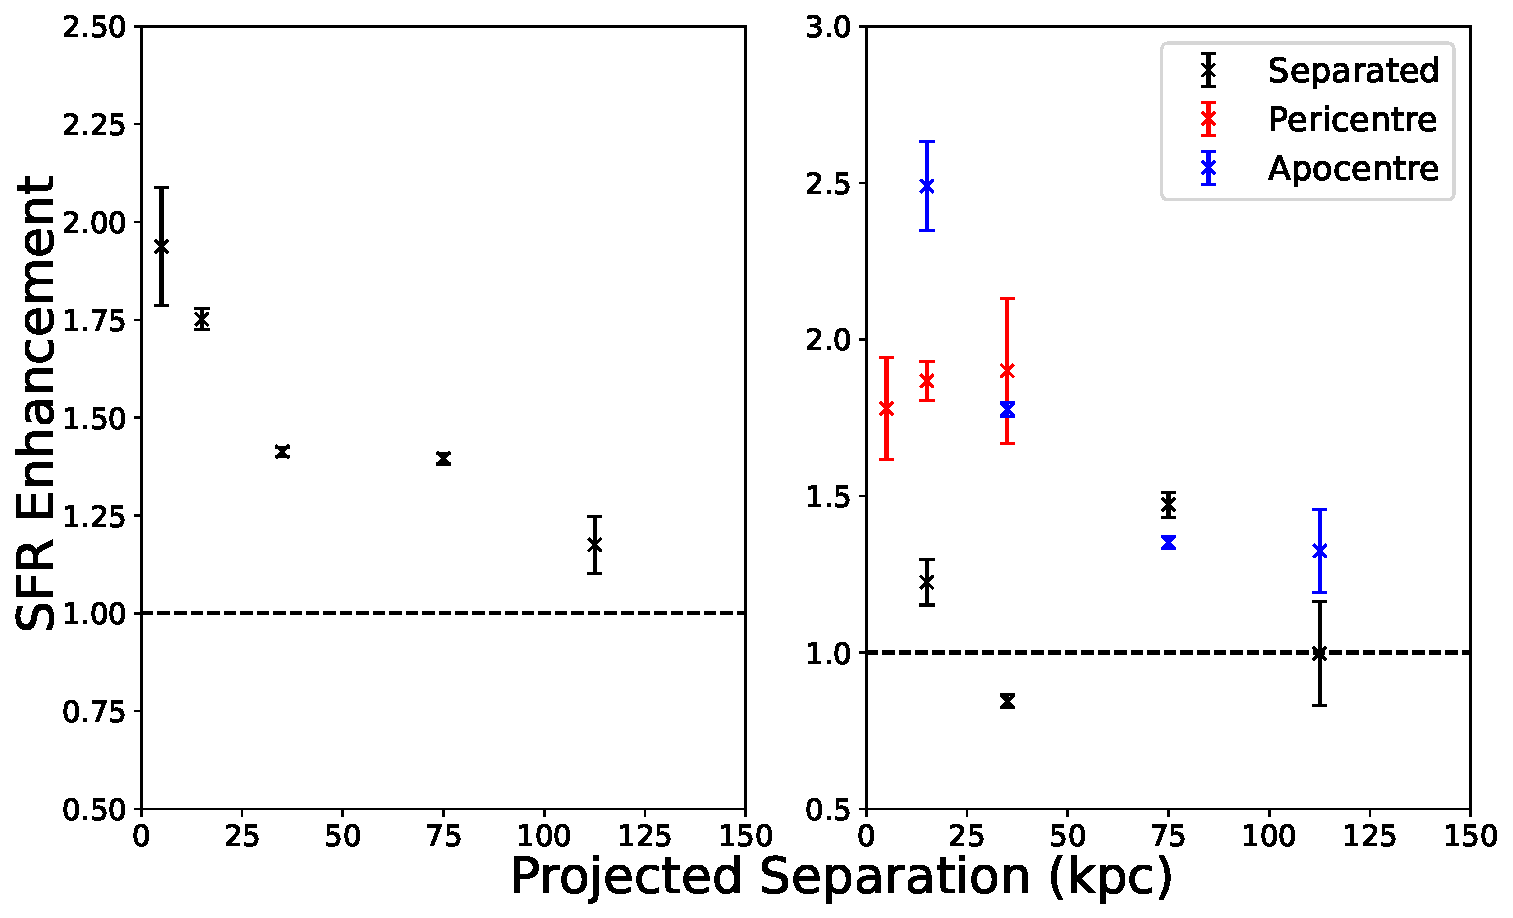
\includegraphics[width=\textwidth]{Chapter3/figures/sfr-enhancement-projected-sep.pdf}
    \caption[The projected separation against the star formation enhancement in average star formation at different bins of projected separation.]{The projected separation against the star formation enhancement in average star formation at different bins of projected separation. Each bin must contain at least 10 counts to be considered. As the bulk of our galaxy pair sample is at low projected separation, we heavily sample from this region of the parameter space. The bins are: [0.5, 10, 20, 50, 100, 125] kpc. As we move to higher projected separation, the bins increase in width to maintain statistical significance in our sample. \textit{Left}: The star formation enhancement found in the entire galaxy pair sample. As expected, we see a gradually decreasing enhancement. \textit{Right}: As left but broken up into different stages of the interaction. Black markers are stage 1, red stage 2 and blue stage 3. We limited our investigation to stages 1, 2 and 3 as only three galaxy pairs were identified in stage 4. We find a generally decreasing star formation enhancement with projected separation but very different individual behaviour dependent on the stage classification.}
    \label{fig:sfr-enhancement-sep}
\end{figure*}

Figure \ref{fig:sfr-enhancement-sep} shows star formation enhancement between our interacting and control binned SFRs and the projected separations between each galaxy pair. On the left of the plot, we have the distribution for the full galaxy pair sample, without taking account of stage. The errors on our measurements are calculated as the standard deviation from the mean within the bin. The dashed black line represents no enhancement in SFR, as the average SFR in the interacting galaxy sample would be equal to the average SFR in the control sample. We find at very small projected separation a SFR enhancement of 1.87 which gradually decreases with projected separation down to approximately 1 at 117.5kpc. 

On the right, we break the galaxy pair sample into different stages and plot out the resultant enhancement in star formation. This shows very different behaviour in enhancement dependent on the stage of the interaction. In stage 1, we find that the star formation is very weakly enhanced, and with no overall structure. The enhancement moves around 1 through the distribution, with some enhancement being a result of low number counts in the bin. Taking into account the errors on our measurements, the true value of the enhancement could be around 1 for the entire projected separation distribution. This is not unexpected. Stage 1 represents when the two galaxies are close pairs, but with no morphological disturbance. Therefore, we would not expect significant, if any, enhancement in the SFR based on the projected separation. This is the stage with the lowest enhancement across projected separation, remaining close to 1.

In stage 2, we see consistent enhancement with projected separation. It is also much larger than stage 1, with it being approximately 1.75 up to 1.90. In fact, the measured enhancement increases across the 50kpc of projected separation. However, accounting for the errors on these measurements and the declining counts in each bin, it is likely that the enhancement does drop as the projected separation increases. We see a very large enhancement in the overlapping stage 3 galaxies which overlap with the stage 2 measurements. The enhancement in stage 3 galaxies then rapidly declines as we move to higher projected separations. After 150kpc, our galaxy pair sample does not have the counts to make robust estimates of the SFE. However, it is important to note that this result has been found with a sample of 960 interacting galaxies in their pairs. No stage 4 galaxies have been represented and in numerous projected separation bins the counts are small enough to have conclusion altering error bars. \textbf{Therefore, it is imperative that future works, with larger sample sizes not only look at the projected separation of the systems but the morphology as well.}

\subsection{Controlling for Galactic Environment} \label{sec:env-cont}
\noindent While we have found clear evidence of evolution in the SFR of interacting galaxies with stage, it is important we remove a potential source of contamination. It is well known that the environment has a direct impact on the observed SFR of galaxies. A galaxy in a cluster environment has, on average, a higher SFR than those in the field \citep{2006MNRAS.373..469B}. Thus, if any of our stage classifications are biased towards one environment or another, it could have severe consequences for our results. Therefore, we utilise the existing COSMOS environment catalogue described in \citet{2017ApJ...837...16D} to ensure there are no environmental biases in our staging. 

Upon applying the matching described in Section \ref{data:environ}, we break our samples into different environment measures with stage. Figure \ref{fig:dens-stage} shows the distribution of our matched samples with their density values. It is important to note that \citet{2017ApJ...837...16D} has a higher mass cutoff than we have implemented in our underlying sample. Therefore, this is showing the density of all systems $\log$M$_*$/ M$_\odot \geq$ 9.6. 

\begin{figure}
    \centering
    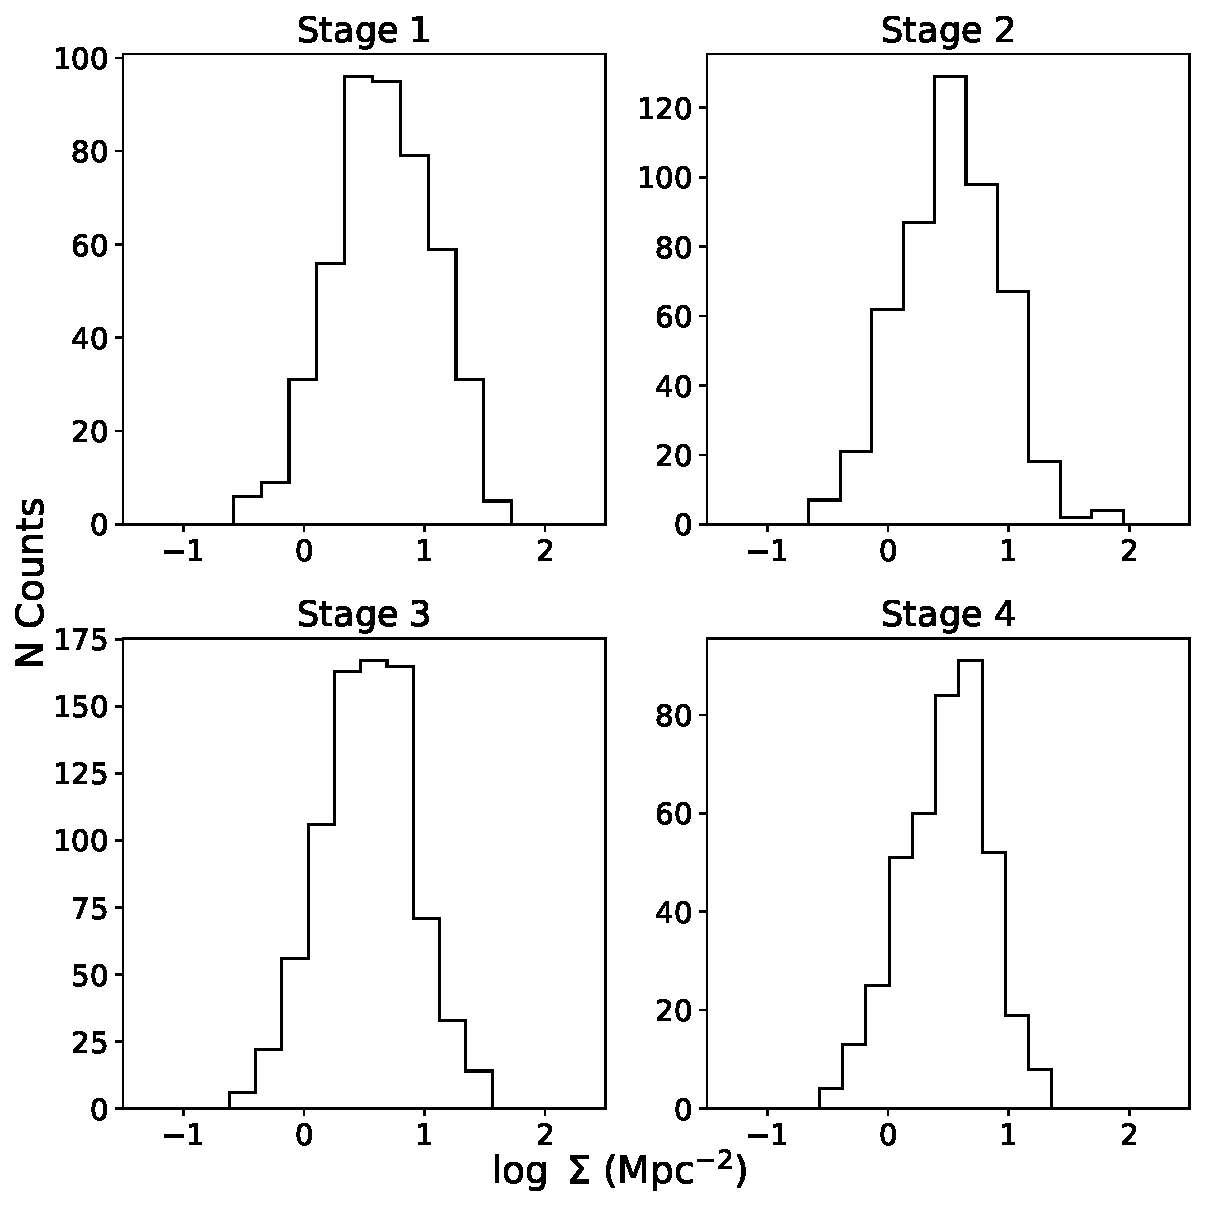
\includegraphics[width=\textwidth]{Chapter3/figures/density-stage.pdf}
    \caption[The density about each of our sources matched with the \citet{2017ApJ...837...16D} catalogue.]{The density about each of our sources matched with the \citet{2017ApJ...837...16D} catalogue. As shown, there is no existing bias in the distribution of galactic environments throughout our stages. This is confirmed by performing KS- and AD-tests. Therefore, we can conclude that the shown evolution in SFR with interaction stage is not due to environmental effects.}
    \label{fig:dens-stage}
\end{figure}

We conduct weighted KS and AD tests on the environment distributions, and confirm they are likely drawn from the same parent sample, with the resultant p-values $\approx$1 the distributions. Thus, there are no biases in our stage selection with environment, and it fair to assume that the evolution in the SFR with stage is due to interaction, not environment.

\begin{figure}
    \centering
    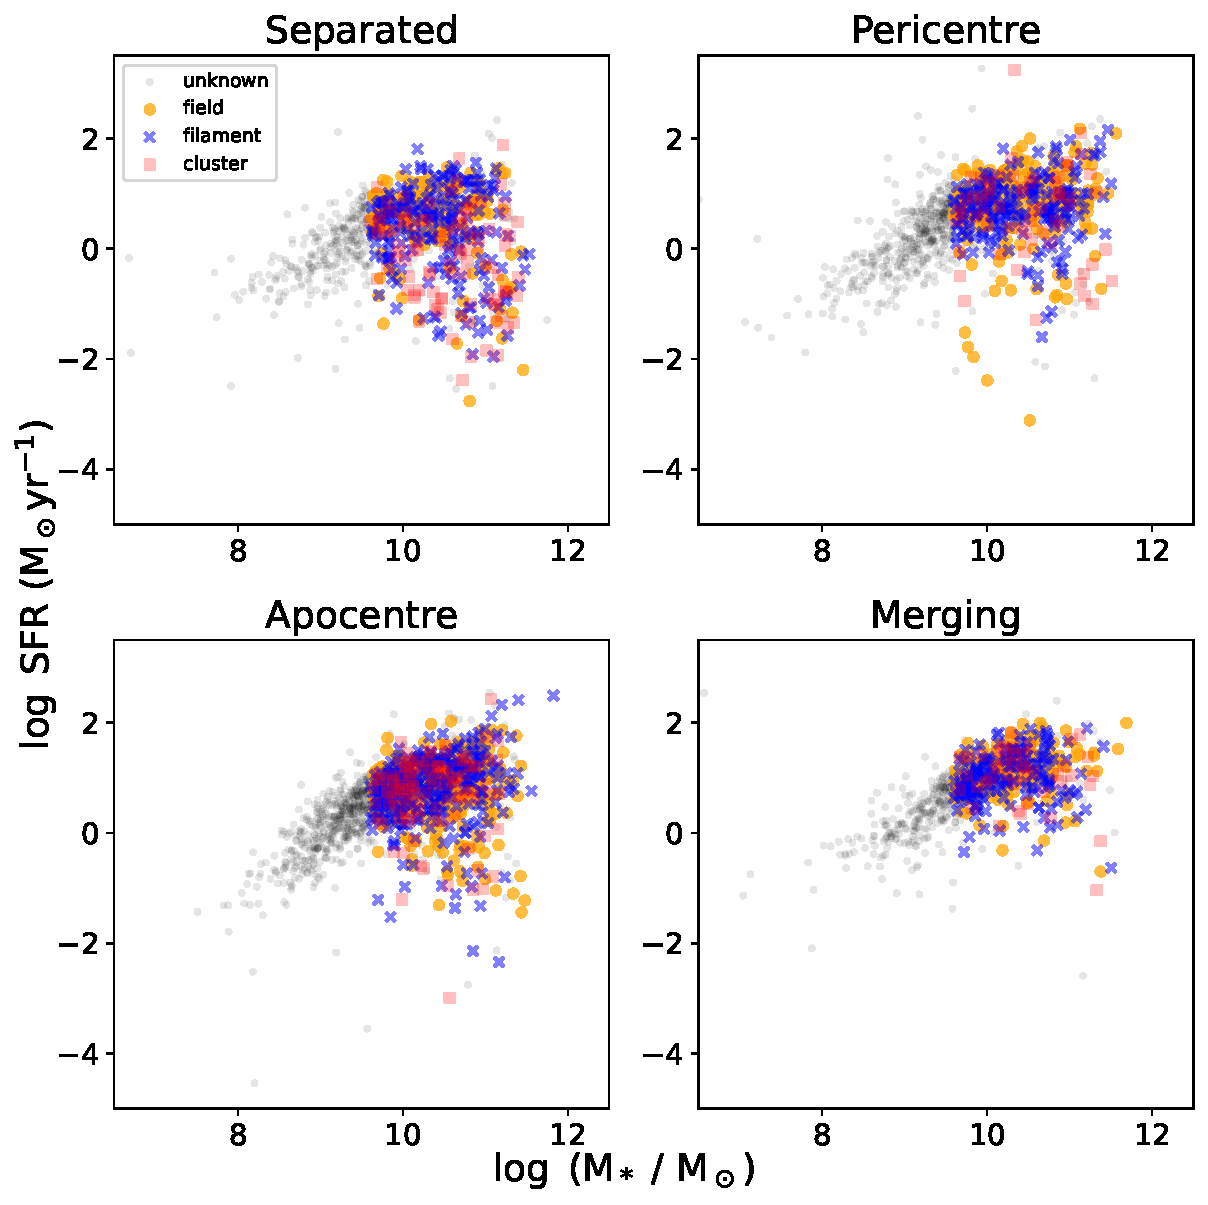
\includegraphics[width=\textwidth]{Chapter3/figures/sfr-mass-density.pdf}
    \caption[The distribution of environment classifications through our sample.]{The distribution of environment classifications through our sample. This is only for sources with a $\log$M$_*$ / M$_\odot \geq$ 9.6. However, from this subsample, we see that there is no trend with environment and that the distribution is random throughout each stage. Therefore, the effects of increasing SFR with interaction stage is not due to environmental effects.}
    \label{fig:dens-sfr-mass}
\end{figure}

Figure \ref{fig:dens-sfr-mass} shows the environment classification in our reduced stellar mass-SFR distribution. This shows that there is no ordered structure, or bias, in our sample with environment and further reinforces that the galactic environment is not responsible for our proposed SFR evolution with stage. The majority of our sample lie either within filaments or in the field. The environment which would have the most effect upon the SFRs of our sample is a cluster environment. However, the fraction of our sample within a cluster is never greater than 10\%. It is important to note, however, that the galaxies most likely to lie in a cluster in our sample would be lower mass galaxies. However, these systems are not found in the red sequence where we see the most change in SFR due to interaction. Therefore, the lack of information here does not have a large impact on this measurement. 

\section{Nuclear Activity with Interaction Stage}\label{results:AGN_stage}
\noindent We now cross match our sample with the two AGN catalogues and methods described in Section \ref{sec:agn-clsf}. This provides us a sample of 1,361 AGN and star forming galaxies (SFGs). The breakdown of number of classifications per stage is shown in Table \ref{tab:agn-sfg-breakdown}. Figure \ref{fig:agn-stage} shows distribution of stellar mass to SFR with stage, with the confirmed AGN and SFGs marked. We find no major changes in AGN with stellar mass or SFR with stage in our sample. Galaxies containing AGN appearing throughout the SFMS and red sequence across each stage. There is no obvious bias in stellar mass or SFR for hosting an AGN. We do, however, see a concentration of AGN in stage 1 on the red sequence at higher masses. This shifts as we increase interaction stage, with the bulk of the AGN beginning to appear at lower masses in stages 3 and 4. Finally, in stage 4 we see AGN and SFGs distributed almost evenly across the star forming main sequence with little bias in distribution with mass. This hints at evolution with stage.

Applying KS- or AD- tests these, however, reveals p-values close to 1 and therefore it is very likely that these distributions have been drawn from the same parent sample. However, due to the low counts of AGN and SFGs in our sample, using KS- and AD-tests to verify this is not optimal. Therefore, we instead investigate the global AGN fractions in our sample across different stages. We apply a weighting, as in our SFR and stellar mass distribution examples, to account for the various counts across the different stages. We then take a second weighting of the measured AGN fraction from the total size of the different samples we have. Thus, we have assumed that we have equivalent counts in each mass bin of our sample as well as approximated having the same sample size in each stage bin.

\begin{figure}
    \centering
    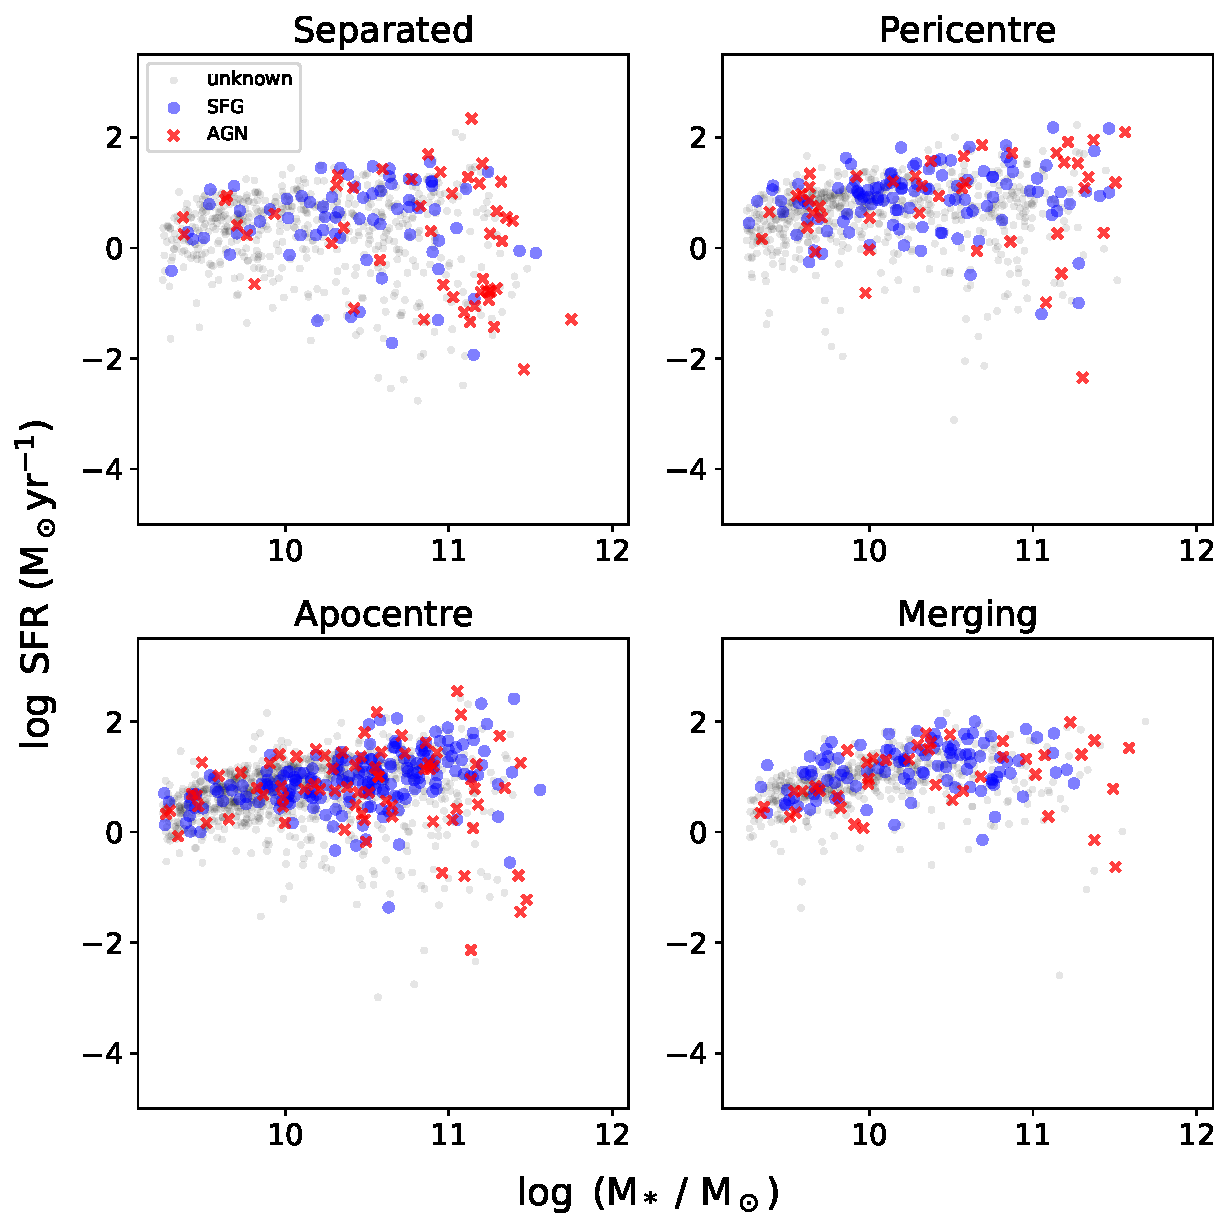
\includegraphics[width=\textwidth]{Chapter3/figures/agn-stage-dist.pdf}
    \caption[The distribution of AGN through stage with SFR and stellar mass.]{The distribution of AGN through stage with SFR and stellar mass. We do not find any major changes and evolution with AGN and SFG position through interaction stage. }
    \label{fig:agn-stage}
\end{figure}

\begin{table}
    \centering
    \begin{tabular}{|c|c|c|c|c|}
		\hline
         & Stage 1 & Stage 2 & Stage 3 & Stage 4 \\
         \hline
        SFG & 135 & 212 & 337 & 199 \\
        AGN & 103 & 117 & 163 & 95 \\
		\hline
    \end{tabular}
    \caption{Breakdown in number of classified AGN and SFGs per stage. With our counts so low in this sample, it is difficult to make concrete conclusions about the evolution of AGN during interaction.}
    \label{tab:agn-sfg-breakdown}
\end{table}

\begin{figure}
    \centering
    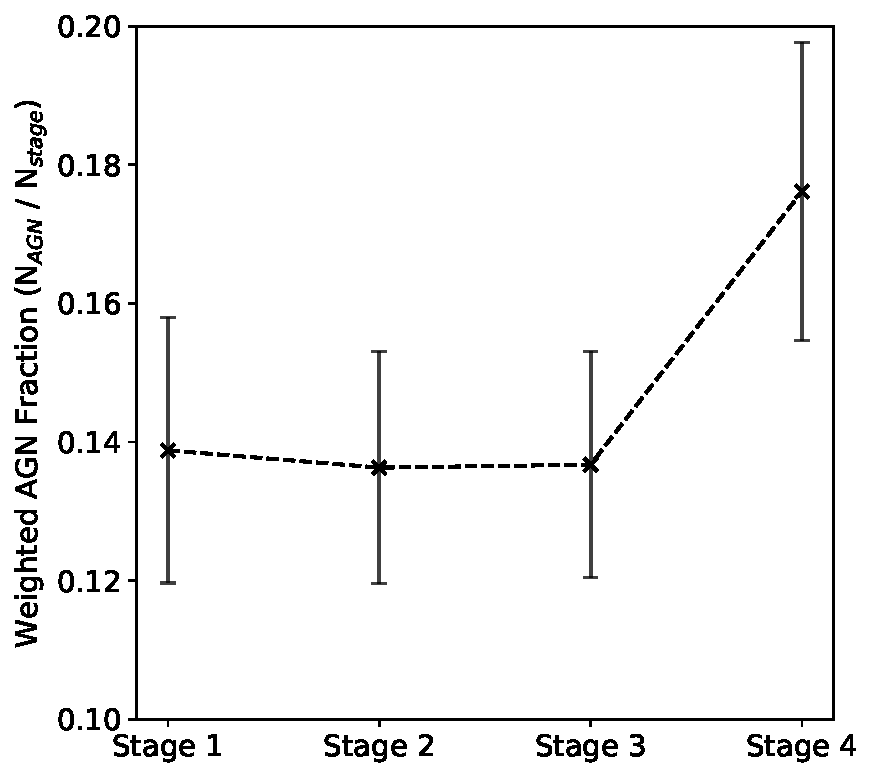
\includegraphics[width=\textwidth]{Chapter3/figures/agn-frac-time.pdf}
    \caption[The change in AGN fraction with stage.]{The change in AGN fraction with stage. We define the AGN fraction as the ratio of number of confirmed AGN divided by the number confirmed AGN and SFGs in the sample. This is then weighted by the relevant sizes of each subsample and the number of unclassified sources in each. Errors on each point are found by bootstrapping. We do not include any sources of which we have no information. We find a sudden drop in AGN fraction from stage 1 to stage 2, followed by a rapid increase from stage 3 to 4.}
    \label{fig:agn-frac-time}
\end{figure}

Figure \ref{fig:agn-frac-time} shows the changing AGN fraction with interaction stage. We find that the AGN fraction generally remains static with stage. There is a small decrease increase from stage 1 to 2, followed by the fraction mostly remaining unchanged until stage 3. Then, in stage 4 we measure a large jump in the AGN fraction. However, before we discuss this result further, we must point out that the large error bars on our measurements and the low number counts of confirmed AGN and SFG make this difficult to interpret. We measure the errors as the standard deviation about the mean in each stage. Thus, while our initial values show relatively little change, because of the large error bars, there could be increase with stage to even a further decline.

% Section here on actually looking at the projected separation of the two systems.
It is also difficult to use interaction stage as a proxy for the projected separation in this context. As shown previously, stages 2 and 3 have some overlap in the range of projected separations we have classified them into. Therefore, we also investigate any overlap between our confirmed pairs and the AGN fractions we see here. We find 104 AGN and 180 SFGs overlap with our confirmed pairs. This sample is far too small to breakdown further into different stages. Therefore, Figure \ref{fig:sfg-agn-proj} shows the change in density of AGN classifications and SFGs with increasing projected separation. As expected, we find that with increasing projected separation the number of confirmed AGN and SFGs decreases. In the AGN distribution, we find two contributing components in it. The first is a peak in the projected separation distribution is from 0kpc-25kpc. The only contribution here is from stage 2 galaxies, which are close to pericentre. The second peak, from a projected separation of 30kpc - 60kpc is dominated by stage 3 galaxies, although some stage 1 AGN are in this peak as well. Finally, the third peak from 85 - 125kpc is representative of a mixture of stage 1 and stage 3 galaxies. None of our stage 4 galaxies which had their secondaries identified overlapped with our AGN and SFG identified sample.

\begin{figure}
    \centering
    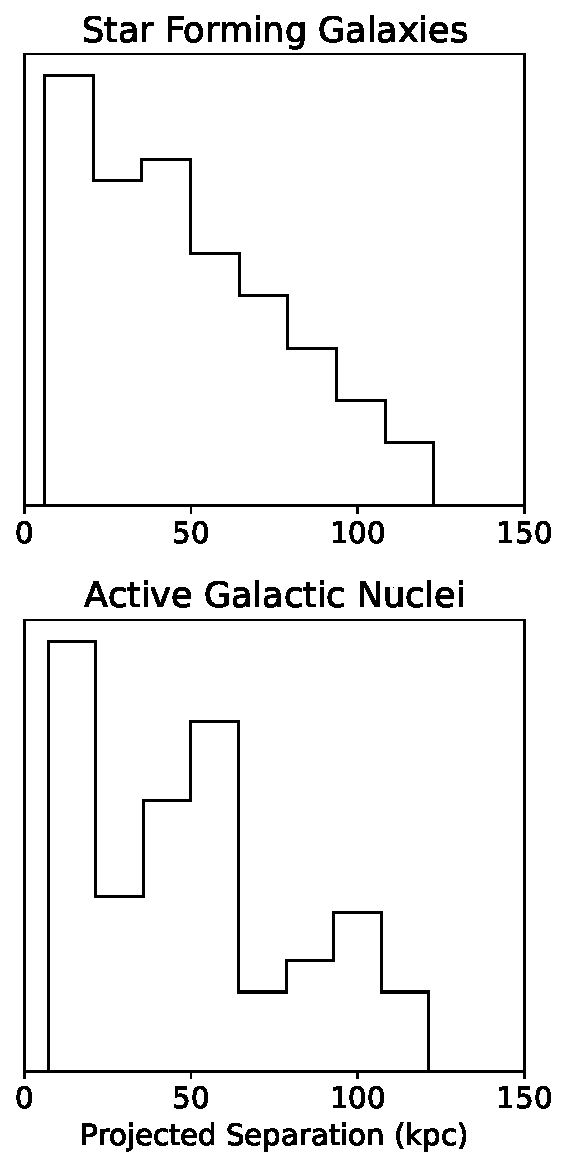
\includegraphics[width=0.58\textwidth]{Chapter3/figures/sfg-agn-dist.pdf}
    \caption[The distribution of both AGN and SFGs which have been cross matched with our confirmed galaxy pairs.]{The distribution of both AGN and SFGs which have been cross matched with our confirmed galaxy pairs. While we find, as expected, the number of AGN and SFGs decreases with projected separation we find an interesting double peak in the AGN sample. The first peak, between a projected separation of 0 and 25kpc is primarily from stage 2 galaxies while the second peak of 40 to 65kpc is of stage 3 galaxies in our sample. As shown in Figure \ref{fig:agn-frac-time}, we expect the fraction of AGN to be similar in these two stages despite being at different parts of the dynamical timescale in interaction. The third peak, from 75 to 125kpc is only from stage 1 and stage 3 galaxies.}
    \label{fig:sfg-agn-proj}
\end{figure}

We find the AGN fraction only increases at the point of coalescence in interaction: stage 4. This indicates that the mechanism driving AGN ignition in interaction is primarily at the point of the closest approach between the two systems. When we investigate the AGN number counts with respect to the projected separation of systems, we find that it gradually declines over the projected separation. However, we find two peaks; first clearly in stage 2 of the interaction where the galaxies are overlapping and secondly in the early parts of stage 3. This could be evidence of a delayed AGN ignition depending on the underlying parameters of the interaction. Thus, \textbf{we find that the AGN fraction is generally unchanged with stage, however, the mechanisms responsible for an increase in the fraction primarily occur when the two systems are actually merging. We find evidence of a delay of ignition, as there is an increase in fraction at a early projected separations in stage 3}.

\section{Discussion}\label{discussion}
\subsection{Interaction Stage and Projected Separation}
\noindent Finding evolution with interaction stage is not a new idea in the field. Multiple works have found increases in SFE and SFR as a function of projected separation of pairs of galaxies \citep{2000ApJ...530..660B, 2008AJ....135.1877E, 2013MNRAS.433L..59P}. Projected separation is often seen as a proxy for the point in the dynamical time of the interaction that is being measured. It is likely that, when the galaxies in the pair are closer together, they are closer to coalescence in the dynamical time and can be thought of as a linear progression in the interaction from being close pairs to coalescence. However, what this fails to capture is the larger complexity of interaction. Without morphological consideration, we are unable to tell whether galaxies at close projected separation are actually about to coalesce or are simply at the closest point of flying by each other.

We find that throughout the different stages of interaction the SFR within the systems is increasing. Observations of interacting galaxies at various stages have found increased gas inflows into the nuclear regions of the galaxies which lead to enhancement in SFR there over their outer reaches \citep{2015A&A...579A..45B}. This is often confirmed with deep observations of individual systems, which capture snapshots of different parts of the dynamical timescale of the interaction \citep{2022MNRAS.514.2769K}. Our study utilises numerous snapshots of the dynamical time of interaction in attempt to build a full picture of the change in SFR. We have found here is that this process of increasing SFR and galaxies being driven to starburst begins from the pericentre of interaction. Multiple simulation works, which have the ability to model the entire dynamical history, show that this is to be expected \citep{2007A&A...468...61D, 2013MNRAS.430.1901H, 2015MNRAS.452.2984K, 2021MNRAS.503.3113M}. Often, these works show an initial dramatic increase in the SFR of interacting systems followed by an exponential decline through the dynamical time before increasing dramatically again at either a second passage or coalescence. \citet{2015MNRAS.448.1107M} is a direct example of this SF history through the merger history.

Our results differ here as we do not find an exponential decrease in the SFR as move from stage 2 systems to stage 3 systems. As stated previously, observational work does support a continued increase in SFE in galaxies to projected separations of out to 80kpc - well into our defined stage 3 systems \citep[for further examples, see][]{2008MNRAS.385.1903L, 2012MNRAS.426..549S}. However, it is important to note that our stage 3 defined classification is a `wide net' that captures many systems that may be very soon after the initial passage in the dynamical timescale. The criteria defining stage 2 and stage 3 are simply that the galaxies must be no longer connected or overlapping morphologically with tidal features. They must only be distinct and separate galaxies. Therefore, our found large enhancement in stage 3 may be from interacting systems which are only just out of the pericentre passage and not enough time has passed for the rapid decline in SFR to begin. 

Nonetheless, we still find a disappearance of the red sequence in stage 3 systems which may come as unexpected to when compared to simulations. It is important to note, however, that this is not the same as saying that a large proportion of the stage 3 systems are classified as starbursting galaxies. While previously mentioned simulations approximate an initial large starburst before rapid decline, we find the interacting galaxy population is pushed being quiescent / sub the star forming main sequence to being on the star forming main sequence. Therefore, it may be more likely that the impact of interaction on star formation is not to suddenly cause rapid star formation in the aforementioned starburst before declining, but rather to gradually increase a galaxy's SFR up and into the blue cloud of galaxies. This could be supported by the surprising lack of rapidly quenched post-interaction galaxies found in both observations \citep{2017ApJ...845..145W} and simulations \citep{2020MNRAS.493.3716H, 2021MNRAS.504.1888Q}. \textbf{Thus, the impact of interaction on star formation is may not be a catastrophic increase in star formation that leads to quenching but, rather, a small increase in galaxies to use whatever gas they have into star formation}. % Expand?

This idea can be brought further forward by considering the large increase in starbursting galaxies we find when going from stage 2 / stage 3 to stage 4 galaxies. Stage 4 represents, in our sample, galaxies that are undergoing the final coalescence of the two systems involved. We find that the point of final coalescence leads to a large increase in the fraction of starbursting galaxies as well as the almost complete disappearance of the quiescent and sub-main sequence fraction of galaxies. Thus, from this result we can conclude that during coalescence galaxies undergo a huge starburst and enhancement in star formation which will quickly lead to their quenching. This is also supported by works such as \citet{2022MNRAS.517L..92E}, which find that galaxies post-coalescence are 30-60 times more likely than control galaxies to have rapidly shut down star formation.

Thus, we can conclude, that for merging galaxies if gas is present within them, star formation will increase and change our classification of the galaxy. We will observe a sudden increase in the star formation rates of these systems followed by a rapid quenching as the gas is used up entirely. This is completely at odds when compared to galaxies that move into stage 3 and do not merge. These stage 3 systems will then slowly lose their enhancement over a long period of time, and return to star forming at their expected rate, whereas only moving into a stage 4 galaxy will lead to a starburst which may incur rapid quenching.

Such a conclusion would also, therefore, explain the often quite large divide in the literature between whether interaction actually leads to enhancement or not. The only part of the interaction which actually causes the enhancement, and is the forking point, is that of stage 2 - where the two galaxies overlap and are at pericentre. From this point, if the galaxies then move off to stage 3 and escape, we will see a gradual decline in the SFE with the stage 3 galaxy only having a minor increase in its star formation classification. Whereas, if the galaxies move into a stage 4 interaction and merge, that is where we see the catastrophic results of a major starburst and the complete using and of all the gas in the systems. Thus, leading to a large fraction of quenched post-merger galaxies, but only after the initial coalescence. 

\subsection{Interaction Stage and AGN}
\noindent The evolution of the AGN fraction in interacting galaxies is similar to that of the evolution of star formation. It has often been found with projected separation the AGN fraction increases. There are multiple observational works that show this \citep{2007MNRAS.375.1017A, 2013MNRAS.435.3627E, 2020ApJ...904..107S} as well as works on cosmological simulations which support these conclusions \citep{2023MNRAS.519.4966B}. In simulations, the increased likelihood of nuclear ignition comes from the sudden increase in gas density in the galactic core which naturally leads to increased black hole accretion and ignition. To satisfy these conditions, actual coalescence of the two systems are required. Observations of interacting galaxies are often interesting, as they contain examples of duel AGN and individual examples \citep[e.g.][]{2017MNRAS.470L..49E, 2021ApJ...923...36S} or investigate the increase in the AGN fraction in only the merger / post-merger stage \citep{2020A&A...637A..94G}.

We find peaks in the AGN fraction with projected separation, before the galaxy merging and coalescence takes place. This is supported with other works which specifically look at AGN fraction with projected separation \citep{2011MNRAS.418.2043E, 2023ApJ...942..107S}. However, we specifically find that the AGN fraction increases rapidly in stage 4 and holds quite constant between stages 1 to 3. This shows, again, shows two distinct effects of interaction which can colour our interpretation of the link between AGN and interaction. It appears, from our results, that the AGN fraction is driven up during the points in the dynamical time when the inner parts of the galaxy are majorly disturbed, and not by the simple movement of gas and dust into the core during the two galaxies passing each other. There is evidence that the onset of nuclear ignition from interaction may be delayed \citep{2011MNRAS.418.2043E}, or even flicker \citep{2015MNRAS.451.2517S} after ignition. Both of these possibilities are reflected distributions of AGN fraction with projected separation.

Again, it is important to note the rather `wide net' that our stage classification takes. There is overlap between our stage 2 and stage 3 classifications at high stage 2 projected separation and low stage 3 projected separations. However, these stages naturally lead onto one another. Therefore, what see in the bi-modal distribution of AGN fraction with projected separation in Figure \ref{fig:sfg-agn-proj} are two peaks. The second of these peaks is at the cross over point of stage 2 to stage 3; the point at which (if the two galaxies have just flown by each other) a delayed AGN ignition could take place. This is also reflected in Figure \ref{fig:agn-stage} where we see a slight increase in AGN fraction in stage 3. This is likely from the ignition of nuclear activity taking place over a large period of time with a delay being involved from the initial flyby.

We also see a dramatic increase in AGN fraction in stage 4 systems, where coalescence is just beginning or has occurred. Multiple works show that this is as expected. \citet{2023MNRAS.519.4966B} has used cosmological simulations to show that we expect a large increase in AGN fraction at coalescence, and even for sometime into the post-merger phase. This is supported by measured AGN fractions in post-merger galaxies. Here, we see that the enhancement actually begins in stage 2, before the coalescence has even begun, but the actual coalescence is what sends it into overdrive. This is matches observations mentioned previously of increased gas densities in nuclear regions and cores, and that stage 4 is when this really occurs in earnest,

However, to more fully study this, we would need a larger sample of confirmed AGN and star forming galaxies from existing photometry or catalogues to make more decisive conclusions based on stage. In this work, we were limited to a small number of AGN and star forming galaxies across each stage. When compared to our paired sample, we do not have the numbers to also divide into stage again. Therefore, Figure \ref{fig:sfg-agn-proj} shows the global AGN number count with projected separation. We show that the two peaks are due to different stages of the interaction, however, these are using very low number counts and should be treated carefully.
 
\section{Conclusions}\label{conclusion}
\noindent In this work, we investigate the evolution of multiple parameters and processes in galaxy interaction with interaction stage. We use the \citet{2023ApJ...948...40O} catalogue of interacting galaxies and cross match it with the COSMOS survey to gain ancillary data. This gives us a sample of 4,135 interacting galaxies of which 960 have a confirmed secondary from available photometric redshift data. We use visual morphology as well as angular separation to split our sample into four distinct stages: (1) close pair, (2) morphologically disturbed and overlapping, (3) morphologically disturbed and distinct, (4) merging. Each stage is designed to capture a different part of the dynamical timescale of the interaction. We then cross match these samples with existing catalogues of environment and active galactic nuclei for further study.

% Stage and SFR
We first split our sample of galaxies into their different stages and investigate their evolution with stellar mass and star formation rate. We conduct Kolmogorov-Smirnov and Anderson-Darling tests to show the mass distribution of our sample does not change with stage, while the star formation rate changes dramatically. This change in star formation rate from stage 1 to 4 is found in the red sequence of galaxies reducing to the point of disappearance. This is further confirmed by sub-classifying each sampled stage into starbursting, main sequence and quiescent galaxies. We find that as the galaxies move from stage 1 to stage 2 the fraction of starbursting galaxies increases while the quiescent galaxy fraction reduces. In stage 4, the starbursting fraction increases dramatically while almost no quiescent galaxies exist in the sample. This implies that the mechanisms responsible for enhancement in star formation in interacting galaxies is dominant from stage 1 to stage 2 and in the final coalescence of the system. We find that, for all of our galaxies, some enhancement in star formation is observed. 

% SFR and projected separation
To further investigate this change in enhancement, we investigate our sub-sample of galaxy pairs and compare it to a mass and redshift matched control sample. We bin our projected separations and measure the ratio between the average interacting SFR and control SFR in each bin. We find, across the whole subsample, a general increase in star formation efficiency as we move to smaller projected separation. The highest found enhancement is below 10kpc. However, when broken down into their constituent stages, we find dramatically different behaviour in the star formation efficiency. This is best seen in stage 2 enhancement, which does not seem to change with projected separation, while there is a dramatic decrease in stage 3 enhancement from 2.5 at 10kpc down to 1.2 at 100kpc. This shows that just using projected separation as a proxy for stage will leave out crucial information to the underlying causes and mechanisms fueling star formation enhancement. To confirm that the effects observed here are not related to biases in the environment, we investigate its relation to our staged sample. We find that the environment is consistent between all stages, with no biases existing.

% Stage and AGN
Finally, we investigate the change in AGN activity across our whole sample. We find that, on average, the AGN fraction remains constant with stage until the point of coalescence. However, when looking at project separation, we find an almost bi-modal distribution. This could be evidence for a delayed ignition in the AGN present in those systems undergoing an interaction. However, it is difficult to draw this conclusion definitively due to small number counts. We also find that the AGN fraction is highest in merging and merged galaxies.

% What does it mean?
While the results with projected separation are not unexpected, those with the different stages are. We have shown that one cannot simply use the projected separation of interacting galaxies as a proxy for the stage of the interaction. We find very different behaviour in the star forming behavior of interacting galaxies based on stage which are at in the dynamical timescale of the interaction. We find the beginning of an enhancement in star formation occurs in stage 2, where the two galaxies are moving past each other at pericentre. Then, through to stage 3, the enhancement remains although with no further increase. There is then another dramatic starburst in stage 4, where the two galaxies actually begin to undergo the merging processes.

% Future Work
Our work shows the importance of considering morphological stage when considering interaction, and that there is a fine interplay between underlying processes and dynamical timescale of an interaction. We require larger samples of correctly staged galaxies to further understand and exploit what these relations are, and how to best investigate when and where star formation and its enhancement occurs. This is also particularly true of the relation between active galactic nuclei and the interaction stage, where we are unable to have the sample size to definitively draw conclusions from our results.
